\documentclass[12pt,oneside,openany]{report}
% Márgenes APA 2.54 cm
\usepackage[a4paper,margin=2.54cm]{geometry}
\usepackage[T1]{fontenc} % mejor codificación de fuentes para español
\usepackage[spanish]{babel}
\usepackage[utf8]{inputenc}
\usepackage{csquotes}
\usepackage{amsmath}
\usepackage{listings}
\lstset{breaklines=true}

\pagestyle{plain}

\usepackage{graphicx}
\graphicspath{{./images/}}
\usepackage{caption}
\usepackage{array}

\usepackage{tocbibind}

\usepackage[normalem]{ulem}
\usepackage{xcolor}
\definecolor{edit30sept}{HTML}{e3256b}

\usepackage{hyperref}
\hypersetup{
    colorlinks=true,
    linkcolor=black,
    filecolor=magenta,      
    urlcolor=black,
    citecolor=black,
}
\urlstyle{same}

\usepackage{microtype}
\usepackage{lmodern} % fuentes vectoriales para evitar error microtype con tamaños sustituidos

% Interlineado APA
\usepackage{setspace}

% Sangría estándar APA 0.5 pulgadas ~ 1.27 cm
\setlength{\parindent}{1.27cm}

% Estilo de referencias APA
\usepackage[backend=biber,style=apa,sorting=nyt,language=spanish]{biblatex}
\DeclareLanguageMapping{spanish}{spanish-apa}
% Workaround: early definition in case apa.bbx \AtEndPreamble hook fails
\providecommand{\datecircaprint}{\bibstring{circa}\printdelim{datecircadelim}}
\addbibresource{references/bibliography.bib}
\addbibresource{references/videography.bib}

% Para regenerar Tabla de contenidos tras un error: `make clean` y luego `make main` (2-3 pasadas automáticas)

% Nota: Para citas con Biblatex apa, usar \parencite y \textcite.

\let\cleardoublepage=\clearpage

\AtBeginEnvironment{quote}{\small}
% Captions en mismo tamaño y doble espacio (controlado por setspace)
\captionsetup{font=normalsize}

% Nombres de listas acorde normativa en español
\renewcommand{\listfigurename}{Lista de Figuras}
\renewcommand{\listtablename}{Lista de Tablas}

\begin{document}
\show\datecircaprint % DIAG: show definition status in log
\show\ifdatecirca % DIAG: show ifdatecirca conditional
\show\biblcstring % DIAG: show biblcstring
\show\printdelim % DIAG: show printdelim

% Safe redefinition avoiding \biblcstring (use \bibstring instead if not yet initialised)
\renewcommand{\datecircaprint}{\ifdatecirca{\bibstring{circa}\printdelim{datecircadelim}}{}} % TEMP PATCH

% Interlineado doble global
\doublespacing

\thispagestyle{empty}
\begin{titlepage}
\renewcommand*{\thepage}{Title}

    \begin{center} 
        \vspace*{3cm}
        
        {\fontsize{16pt}{22pt}\selectfont\textbf
            {Significación social y supervivencia simbólica en la producción de imagen artística sobre la resistencia y crisis del Hospital San Juan de Dios, Bogotá, 2000-2015}
        }


        
        \vspace{1.5cm}
        
        \text{Por:}
        
        \vspace{0.5cm}
        
        	JUAN CARLOS ARROYO SOSA, B.A. \\

        \vspace{1.5cm}
        
        	Tesis presentada a la Facultad de Artes y Humanidades \\
            de la Universidad de Caldas, en cumplimiento parcial de los requisitos \\
            para el grado de Magister en Diseño y Creación Interactiva

        
        \vspace{2.5cm}
        
        Asesora de Tesis:\\

        \vspace{0.5cm}
        
        BEATRIZ DEL CARMEN PERALTA DUQUE, Phd.\\
        
        \vspace{3cm}
        
            Universidad de Caldas\\
            \vspace{0.5cm}
            Artistic-2.0 license 2024. 
    
    \end{center}

\end{titlepage}
\cleardoublepage

\pagenumbering{roman}
\setcounter{page}{1}

\phantomsection
\addcontentsline{toc}{chapter}{Declaración de ética}
\section*{Declaración de ética}
\setlength{\parskip}{1em}

Yo, quién escribe este texto, he sido durante años un silencioso observador de el caso del San Juan, y como afectado contiguo al drama social derivado de la crisis y fin de los servicios hospitalarios, he visto los síntomas de decadencia funcional, deterioro de las edificaciones, y el drama humano vivido por las personas alrededor de la persistencia en las distintas formas de resistir al fin del HJSD. Una de esas trabajadoras a las que aún se les adeuda su liquidación, es mi madre, la enfermera Berenice Sosa o como aún después de tantos años de no ejercer su profesión, sus compañeras del San Juan le siguen diciendo “jefe Berenice”.

Esta investigación titulada \textit{Significación social y supervivencia simbólica en la producción de imagen artística sobre la resistencia y crisis del Hospital San Juan de Dios, Bogotá, 2007-2017} se ha realizado respetando los principios éticos fundamentales de integridad, transparencia y respeto hacia las personas y los materiales involucrados.  

La recolección de datos incluyó el uso de material de registro de obra artística, consulta bibliográfica, así como registro fotográfico personal y cedido temporalmente para consulta por ex trabajadores del hospital, quienes colaboraron de manera voluntaria y con su consentimiento informado. Se garantizó la confidencialidad de los participantes y el uso adecuado de los recursos proporcionados, asegurando que sus contribuciones fueran tratadas con el mayor respeto y se emplearan exclusivamente con fines académicos y de investigación.  

El estudio busca promover la comprensión de las dimensiones simbólicas y sociales de la resistencia y crisis del Hospital San Juan de Dios, contribuyendo a preservar su memoria histórica. Se evitó cualquier manipulación de la información recopilada y se actuó con responsabilidad frente a los derechos de los artistas, autores y participantes involucrados en este proceso.  

Esta tesis se adhiere a los principios éticos de la investigación académica y se compromete a actuar en beneficio de la verdad, el conocimiento y el reconocimiento cultural. 
\pagebreak

\phantomsection
\addcontentsline{toc}{chapter}{Resumen}
\section*{Resúmen}
\setlength{\parskip}{1em}

El propósito de esta investigación es la construcción de sentido a través de la imagen sobre el caso de crisis y resistencias del Hospital San Juan de Dios, Bogotá. Se propone apelar a la imagen como vestigio y sustrato dialógico del imaginario social sobre las profundas transformaciones en el sistema público de salud colombiano que ocasionaron el entramado sistémico de problemáticas sociales complejas. Es una crisis en la cual al menos 3.640 personas quedaron desempleadas, y aproximadamente a 1.500 trabajadores no se les pagó la liquidación por sus años de trabajo, con severas consecuencias en el bienestar de estas personas, desencadenando además un drama y abandono social y estructural que no fue ajeno a la mirada artística, cultural y patrimonial.

Esta investigación se sustenta en los campos antropología de la imagen, estudios visuales y socio semióticos, para crear un fundamento argumentativo que permita «trabajar» con imágenes, que es en esencia, pensar a través de las imágenes.

El alcance es apropiar prácticas metodológicas que permitan el análisis de aspectos del fenómeno de crisis, a través de la interpretación de imagen. Así, se hace una apropiación de la idea de montaje complementado con algunos pasos de enunciación de imaginarios sociales y estructuras semióticas llamadas imágenes-síntoma y anacronismos, para luego recurrir a la capacidad del observador como mediador entre la imagen y el discurso.

\vspace{1cm}
\textbf{Palabras clave:} imagen-síntoma, resistencia social, memoria colectiva, crisis hospitalaria, semiótica visual, antropología de la imagen.
\pagebreak



\phantomsection
\addcontentsline{toc}{chapter}{Dedicatoria}
\section*{Dedicatoria}

\vspace{2cm}

A todas las personas, vivas o que nos han dejado, a todas aquellas que han sido tocadas en su alma o en su salud por las cargas de la vida laboral, que han luchado incansablemente por sus derechos y por preservar el espíritu del cuidado humano, recordándonos la importancia de la dignidad y el bienestar de cada ser humano.

\vspace{4cm}

\subsection*{Agradecimientos}
A mi esposa, quien me ha acompañado con amor y paciencia en este proceso; a mi madre, cuyo ejemplo de lucha y resistencia ha sido una inspiración constante; a mis profesores y tutores; y a todas las personas que, de una forma u otra, contribuyeron a la realización de este trabajo. Su apoyo ha sido un pilar fundamental a lo largo de este viaje, especialmente en los momentos en que las dificultades de la vida hicieron que observar y escribir se convirtieran en un refugio y una fuente de alivio.
\pagebreak

\phantomsection
\addcontentsline{toc}{chapter}{Licencia}
\section*{Licencia}

Esta tesis está licenciada bajo los términos de la licencia \textbf{Creative Commons Atribución-NoComercial-CompartirIgual 4.0 Internacional (CC BY-NC-SA 4.0)}, lo que permite a cualquier persona:

\begin{itemize}
    \item Copiar, redistribuir y adaptar la obra en cualquier medio o formato.
    \item Crear obras derivadas con fines no comerciales, siempre que se reconozca adecuadamente la autoría original y se indique si se han realizado cambios.
    \item Distribuir las obras derivadas bajo la misma licencia (CC BY-NC-SA 4.0).
\end{itemize}

\subsection*{Términos de la Licencia}

Al hacer uso de esta obra, aceptas que:

\begin{itemize}
    \item Debes otorgar el crédito correspondiente al autor, proporcionar un enlace a la licencia e indicar si se realizaron cambios.
    \item No puedes utilizar el material con fines comerciales.
    \item Si remezclas, transformas o construyes a partir del material, debes distribuir tu contribución bajo la misma licencia que el original.
\end{itemize}

Para consultar el texto completo de la licencia, visita:  
\href{https://creativecommons.org/licenses/by-nc-sa/4.0/deed.es}{creativecommons.org/licenses/by-nc-sa/4.0/deed.es}

\subsection*{Aclaración sobre fotografías y registros de obras}

Las imágenes y registros visuales incluidos en esta tesis —en particular aquellas compartidas por las extrabajadoras del Hospital San Juan de Dios (HSJD) y citadas en el texto— \underline{pertenecen a sus respectivos autores y mantienen sus propias licencias de uso}.

Dichos materiales \textbf{no} están cubiertos por la licencia Creative Commons de esta tesis. Para cualquier uso, reproducción o distribución de estas imágenes, se recomienda contactar directamente a los autores o titulares de derechos para conocer sus condiciones específicas.



\renewcommand{\contentsname}{Tabla de contenidos}
% Nota: compilar al menos 2 veces para regenerar TOC después de cambios.
\cleardoublepage
\phantomsection
\tableofcontents
\newpage

\pagenumbering{arabic}
\setcounter{page}{1}

\chapter{Conceptualización del problema}
\section*{Introducción al fenómeno}

\textcolor{edit30sept}{Mi aproximación al Hospital San Juan de Dios no surge de una distancia académica convencional, sino de una intimidad familiar que inicialmente me mantuvo en una posición de “observador silente”. Esta condición particular, lejos de constituir una limitación metodológica, se revela como una perspectiva necesaria para comprender las complejidades visuales y emocionales del caso. Como señala Etienne Samain en su reflexión sobre el trabajo con archivos fotográficos, “acepta el desafío de efectivamente crear mecanismos originales de trabajo con las imágenes en la dirección de una anamnesis de su propia experiencia visual” (Samain, 2016, p. 116). En mi caso, esta anamnesis personal se convierte en herramienta epistemológica fundamental.}

\textcolor{edit30sept}{El vínculo directo con el San Juan —mi madre fue trabajadora del hospital— me posicionó inicialmente en lo que denomino un “pudor investigativo”: una resistencia ética a “meter la mano” en un conflicto que transformaba radicalmente la vida de las personas más cercanas. Este pudor, que posteriormente comprendí como una forma de respeto hacia la complejidad del fenómeno, se transformó gradualmente en curiosidad metodológica. La observación del cambio profundo en el estilo de vida de mi madre, su decisión moral y ética de formar parte del proceso de resistencia, me reveló que en el San Juan ocurrían eventos que demandaban “una mirada crítica” más allá de lo meramente político o laboral.}

\textcolor{edit30sept}{La investigación tomó un giro definitivo cuando Margarita Castro me ofreció acceso a su archivo personal —“sus discos, sus imágenes, sus fotografías”— en un gesto que Samain describe perfectamente: “ella no lo llama archivo, sino me comparte”. Este momento marca lo que podríamos denominar un “encuentro con la imagen del San Juan”: la búsqueda de respuestas en el “adentro” del hospital se resolvió en “otro momento, en otro espacio, en otro lugar, en otra materialidad que es en los archivos digitales y en los archivos físicos de Margarita”.}

\textcolor{edit30sept}{Como establece Samain en su metodología de trabajo con archivos visuales, el investigador debe preguntarse: “¿qué se pretende hacer de un archivo, cuáles serán sus destinos? ¿Para quién, como y por qué?” (Samain, 2016, p. 116). En el caso del archivo de Margarita, me encontré ante “una colección sin colección, un archivo sin archivo”: una mezcla de miradas que incluía tanto “la mirada de quien registra su propia historia” como “la mirada de quien indaga”. Esta multiplicidad de perspectivas contenidas en un mismo corpus visual evidencia lo que Samain denomina la “potencia” de las imágenes para hacer emerger significados que trascienden la intencionalidad original del registro.}

\textcolor{edit30sept}{El descubrimiento crucial fue comprender que “la imagen emerge no por capricho, sino porque la imagen está ahí latente, la imagen finalmente emerge ante el atractor de la mirada”. En el trabajo de artistas como David Lozano en su obra Hortúa Inhospitalaria (véase Figura~\ref{fig:david_lozano_hortua}), pude observar cómo confluían múltiples dimensiones: “el drama social, el drama laboral, también como la profundidad digamos del abandono arquitectónico, patrimonial, el tema del cuidado humano, el tema del cuerpo”. Esta confluencia reveló que las manifestaciones visuales y estéticas no eran superficiales, sino que operaban como condensadores de complejidades sociales más profundas.}

\begin{figure}[p]
    \thispagestyle{empty}
    \captionsetup{labelformat=empty,textformat=empty}
    \begin{tikzpicture}[remember picture,overlay]
        \node[inner sep=0pt] at (current page.center) {
            \includegraphics[height=\paperheight]{hortua-inhospitalaria.jpg}
        };
        \node[anchor=south,text width=0.85\paperwidth,align=center,fill=white,fill opacity=0.9,text opacity=1,inner sep=15pt] at ([yshift=3cm]current page.south) {
            \small \textbf{Figura 1.1:} Hortúa Inhospitalaria, 2017. Performance de David Lozano.\\[0.3em]
            \href{https://david-lozano.org/work/hortua-inhospitalaria}{Copyright David Lozano}
        };
    \end{tikzpicture}
    \caption{Hortúa Inhospitalaria, 2017. Performance de David Lozano.}
    \label{fig:david_lozano_hortua}
\end{figure}

\textcolor{edit30sept}{Samain afirma que “las imágenes, esa colección, ese conjunto de archivos digitales con intención, que tienen una intención, eso genera como una potencia que permite, aún estando en otro momento, en otro tiempo, en otro contexto, volver a ellas y mirarlas” (Samain, 2016, p. 105), en el archivo de Margarita funciona precisamente como este tipo de “conjunto con intención”. Las operaciones de montaje —poner “una imagen con otra”— revelan narrativas no explícitas, pero profundamente significativas, sobre las condiciones de habitabilidad, resistencia y supervivencia en el hospital.}

La crisis del Hospital San Juan de Dios (HSJD) emerge como un laboratorio social donde el diseño y la creación interactiva permiten explorar las dinámicas de transformación institucional, memoria colectiva y resistencia ciudadana. Este estudio trasciende la mera indagación documental o artística para analizar cómo diversas acciones simbólicas, argumentales y estéticas evidencian una intensa producción visual en torno a dicha crisis. Los registros de estas acciones configuran un corpus de imágenes que posibilita interpretar tanto los síntomas visuales de la crisis sistémica como el deterioro arquitectónico y patrimonial en su interacción con el drama humano y social.

El caso del HSJD resulta emblemático en el contexto de las crisis institucionales derivadas de las transformaciones masivas en los sistemas de salud pública. Surge entonces la pregunta: ¿cómo comprender, explicar e interpretar los registros visuales y las obras que actúan como evidencias del drama humano y de la defensa de un bien público?

\textcolor{edit30sept}{Estas evidencias, que denominamos imagen-síntoma, constituyen presencias disruptivas que irrumpen en el curso \textcolor{edit30sept}{normativizado} de la representación visual. Se trata de supervivencias, latencias y reapariciones que habitan las imágenes y desafían el régimen escópico dominante: una mirada que se torna paisaje contemplativo y desvincula la acción crítica. La metodología aplicada a esta colección visual de memoria social permite abordar el fenómeno a través de la imagen, generando un espacio para interpelar y activar la percepción más allá de lo meramente representacional.}

El concepto de imagen-síntoma\footnote{\begin{quote}La idea de la imagen como síntoma, tomada por Didi-Huberman de Freud y aplicada al campo de la historia del arte, reconoce las diferencias entre disciplinas y experiencias. Sin embargo, el uso del carácter sintomático de la imagen en la historia del arte mantiene paralelismos con el análisis de los sueños, aunque aquí se utiliza para nombrar la perturbación que lo visual causa dentro de lo visible \parencite[p. 37]{VegaArevalo2017}\end{quote}} resulta fundamental para comprender cómo las representaciones visuales del HSJD trascienden la mera documentación para convertirse en manifestaciones de tensiones sociales más profundas. Como señala Didi-Huberman:

\begin{quote}
Si la imagen es un síntoma —en el sentido crítico y no clínico del término—, si la imagen es un malestar en la representación, es porque indica un futuro de la representación, un futuro que no sabemos aún leer ni, incluso, describir \parencite[p. 177]{DidiHuberman2011}.
\end{quote}

Este estudio profundiza en el papel de la imagen como medio privilegiado para la contemplación de los fenómenos sociales, ofreciendo nuevas perspectivas que contribuyen al debate sobre el rol del arte y el diseño en los procesos de cambio social y en la construcción de memoria colectiva.

El diseño, entendido como práctica crítica y performática, permite develar las capas de significado ocultas en los registros visuales. No se trata únicamente de documentar, sino de construir narrativas que revelen las tensiones sociales subyacentes. Las imágenes del HSJD se transforman así en interfaces de memoria, donde cada fragmento, ruina y registro artístico opera como un nodo de información compleja.

\textcolor{edit30sept}{En este marco, se propone el concepto de \textit{meta-composición estética y documental} para nombrar el tránsito del análisis de la imagen al dispositivo que la contiene y la reescribe críticamente. Se concibe como una operación de segundo orden que, mediante el \textit{montaje}, articula archivos, escenas, anacronismos e \textit{imagen-síntoma} en una composición que reflexiona sobre su propio proceso de documentación y producción de sentido. Esta operación no busca clausurar significados, sino activar la experiencia crítica del lector/espectador, integrando procedimientos de archivo, selección y montaje en un continuum estético-documental coherente con los objetivos de esta investigación.}

\textcolor{edit30sept}{Desde esta perspectiva, el diseño se concibe como una herramienta estratégica para articular un dispositivo de activación memorial: un mecanismo que, a través de obras artísticas y registros visuales, cataliza procesos orientados a:}

\begin{itemize}
\item Desarticular las narrativas oficiales sobre el abandono institucional;
\item Visibilizar las experiencias de trabajadores y comunidades afectadas;
\item Generar nuevas formas de comprensión y elaboración del conflicto social.
\end{itemize}

\textcolor{edit30sept}{En el ensayo \textit{El derecho a mirar}, Nicholas Mirzoeff define la visualidad no como una mera percepción óptica, sino como un conjunto de relaciones que combinan la información, la imaginación y la reflexión para generar un panorama tanto físico como psíquico. Esta concepción desborda el sentido técnico de “ver” y la aproxima a una práctica discursiva que produce realidad al articular formas de conocimiento, afecto y poder. Desde esta perspectiva, dichas tres dimensiones pueden entenderse como \textit{métodos de visualización}, en tanto configuran operaciones epistemológicas mediante las cuales se construyen modos de percepción, interpretación y representación del mundo.}

\begin{quote}
\textcolor{edit30sept}{A pesar de su nombre, la visualidad no está únicamente compuesta por percepciones visuales en un sentido físico, sino que engloba un conjunto de relaciones en las que se combinan la información, la imaginación y la reflexión para generar un panorama tanto físico como psíquico \parencite{Mirzoeff2016}.}
\end{quote}


\textcolor{edit30sept}{La información, la imaginación y la reflexión operan aquí como tres métodos de visualización interdependientes que orientan el desarrollo analítico de esta investigación. Nombrarlas métodos implica reconocer su carácter procesual y activo: no describen únicamente lo que la visualidad contiene, sino cómo se produce. La información organiza y materializa los datos visibles; la imaginación interviene como potencia de creación y recomposición de lo real; y la reflexión introduce la distancia crítica que permite reconfigurar la mirada y cuestionar los regímenes de visibilidad establecidos. Así, estos tres métodos de visualización atraviesan el análisis propuesto en esta investigación, orientando la lectura de las imágenes no como objetos estáticos, sino como campos de experiencia donde se interrelacionan el conocimiento, la sensibilidad y la crítica.}

\textcolor{edit30sept}{Más que categorías cerradas (la información, la imaginación y la reflexión), constituyen dinámicas de pensamiento y percepción que atraviesan los distintos niveles de lectura del archivo visual del HSJD. En este sentido, la imagen-síntoma se concibe como un espacio donde estos procesos convergen, permitiendo que la representación trascienda su dimensión documental para devenir en una herramienta de interpelación al régimen escópico dominante.}


\section*{Contextualización histórica}

El Hospital San Juan de Dios (HSJD) de Bogotá, fundado en 1723, se estableció como un centro pionero de atención médica y asistencia social para la población vulnerable. Durante casi tres siglos, esta institución se consolidó como un referente fundamental de la salud pública en Colombia, destacándose tanto por su labor asistencial como por su rol en la formación de profesionales de la salud. Sin embargo, la década de 1990 marcó el inicio de una serie de crisis institucionales y financieras que culminarían en su cierre.

El año 2001 representa un punto de inflexión en la historia del hospital, cuando "3.640 personas quedaron desempleadas, y aproximadamente 1.500 trabajadores no recibieron la liquidación correspondiente por sus años de servicio" \parencite{Castiblanco2017}. Este acontecimiento catalizó múltiples formas de resistencia ciudadana que trascendieron la mera reivindicación laboral, evidenciando un complejo entramado de problemáticas sociales.

La crisis del HSJD tiene raíces profundas que anteceden al cese de sus operaciones. Según el investigador Mario Hernández, especialista en historia de la medicina, las décadas de 1970 y 1980 marcaron el inicio de la crisis de los Estados de Bienestar, período caracterizado por la implementación de políticas neoliberales. La presión por incorporar los servicios de salud a las dinámicas de mercado impulsó una transformación institucional que el hospital, originalmente concebido bajo un modelo de beneficencia, no logró asimilar exitosamente. Esta transición fallida se manifestó en el deterioro progresivo de su infraestructura patrimonial, aunque el hospital mantuvo su función asistencial hasta su último día de operación.

Paralelamente a las iniciativas institucionales para su reapertura, emergieron diversas expresiones de resistencia social, manifestaciones artísticas y acciones conmemorativas que abordaron la complejidad del fenómeno. Esta investigación se centra en el análisis de la construcción de sentido a través de obras e imágenes artísticas, estéticas y poéticas no funcionales.

\subsubsection*{Exhibición y creación}

El HSJD se ha convertido en un punto focal para diversos campos disciplinares, atrayendo la atención de urbanistas, antropólogos y artistas plásticos, quienes encuentran en sus espacios un rico territorio para la reflexión y la creación. Este caso paradigmático ha catalizado el debate público sobre la salud como derecho fundamental, manifestándose a través de diversas prácticas disciplinares y expresiones simbólicas.

A partir de 2007, se observa una proliferación sistemática de manifestaciones artísticas que abordan explícitamente la problemática del HSJD. Desde entonces, se han producido y exhibido con regularidad casi anual obras artísticas, intervenciones estéticas y ocupaciones arquitectónicas relacionadas con esta situación.

\begin{table}[htbp]
\centering
\begin{tabular}{|l|l|l|}
\hline
\textbf{Año} & \textbf{Artista} & \textbf{Obra} \\ \hline
2007 & María Elvira Escallón & En estado de coma \\ \hline
2011 & Nicolas Van Hemelryck & San Juan sin Dios \\ \hline
2013 & Juan Camilo Ahumada & Tiempo de dios (guión para teatro) \\ \hline
2015 & Fredy Alzate & Quiste \\ \hline
2015 & Alexandra Mccormick & Potenciales Evocados para aplicaciones clínicas \\ \hline
2015 & Víctor Garcés & Juan N de Dios \\ \hline
2015 & Jenniffer Duarte & Didácticos para una sala de espera \\ \hline
2015 & Ana Karina Moreno & Una más de las resistencias \\ \hline
2015 & Nathaly Rubio & Lo mejor es que nos olvidamos \\ \hline
2015 & Harold Ortiz & Sala de espera \\ \hline
2015 & Alejandro Arango & Egotherapy \\ \hline
2015 & David Lozano & Hortua inhospitalario \\ \hline
2017 & Luisa Fernanda Vela & Al margen \\ \hline
\end{tabular}
\caption{Obras y artistas relacionados con el HSJD, 2007-2017.}
\label{tabla:obras_artistas}
\end{table}

Complementando estas obras, se han realizado diversas activaciones in situ, incluyendo la \textit{Cumbre Mundial de Arte y Cultura para la Paz} y \textit{Time Bag Bogotá} \parencite{IDARTES2015}. Esta tendencia ha continuado más allá del marco temporal de este estudio, con eventos como la \textit{Feria del Millón} (2021), \textit{Siga esta es su casa} (2022) y \textit{La pulsión de la vida} - Activaciones sociales del IDPC.

\section*{Planteamiento del problema}

La crisis del Hospital San Juan de Dios (HSJD) de Bogotá plantea interrogantes fundamentales sobre la respuesta social ante el abandono institucional: ¿Qué acciones tomar? ¿Permanecer, partir, resistir? ¿Por qué y hasta cuándo? Si bien el egreso del último paciente en 2001 marcó un hito significativo, este evento no representó el cierre definitivo del hospital. El proceso de deterioro institucional había iniciado años antes, y las gestiones para su liquidación y eventual reapertura se han extendido por décadas, situando al HSJD en un peculiar estado de latencia activa.

Paralelamente a los esfuerzos institucionales, el HSJD ha sido escenario de diversas manifestaciones de resistencia social, investigación académica y expresión artística que abordan la complejidad del fenómeno. Mientras el hospital experimentaba su desmaterialización funcional, emergían simultáneamente acciones de construcción de sentido en sus dimensiones patrimoniales, estéticas y poéticas. Este contexto suscita interrogantes cruciales sobre la naturaleza de la imagen artística y su capacidad para expresar la crisis y resistencia en el HSJD.

Para analizar los registros gráficos y audiovisuales —que incluyen procesos de creación artística, instalaciones \textit{in situ}, performances y una obra de dramaturgia— se adopta el concepto de \textit{imagen-síntoma}. Este enfoque trasciende el análisis formal de las imágenes para examinar su capacidad de revelar manifestaciones del drama humano y social, considerando que estos registros contienen signos icónicos e indicios de la imaginación social colectiva.

El \textit{corpus} de imágenes relacionadas con el HSJD exhibe recurrencias discursivas provenientes de diversos ámbitos de participación, evidenciando tanto la crisis como las respuestas críticas ante situaciones que generan más interrogantes que certezas. Estas representaciones visuales constituyen un discurso que demanda una interpretación desde una perspectiva crítica y multidimensional.

En este contexto, surge la pregunta central: ¿De qué manera las representaciones visuales y artísticas de la crisis del HSJD contribuyen a la construcción de la memoria colectiva y al entendimiento de problemáticas sociales sistémicas? ¿Cómo pueden estas representaciones ser reinterpretadas, mediante el montaje y la experiencia visual, para generar narrativas transformadoras que estimulen el debate social?. \textcolor{edit30sept}{Metodológicamente, la \textit{meta-composición estética y documental} opera como respuesta al problema de investigación: permite reconfigurar el \textit{corpus} visual en escenas montadas que hacen visible el \textit{síntoma} y el \textit{anacronismo} como tensiones productivas, habilitando una construcción de sentido que excede la mera acumulación de evidencias y propone una forma reflexiva de organización de la memoria visual.}

De esta interrogante principal se desprenden tres preguntas orientadoras:

\begin{enumerate}
    \item \textbf{¿Cómo se representa la crisis y la resistencia en el HSJD a través del arte y la memoria visual?}

    \item \textbf{¿Qué significado adquiere la imagen artística en el contexto de crisis social y resistencia?}

    \item \textbf{¿Cómo las obras visuales sobre el HSJD establecen una relación simbólica entre el entorno social y el espectador?}
\end{enumerate}

\section*{Justificación y relevancia}

La crisis del Hospital San Juan de Dios (HSJD) constituye una problemática sistémica donde convergen múltiples dimensiones interconectadas: económicas, administrativas, sociales, políticas y culturales. Desde la perspectiva del diseño y la creación interactiva, resulta pertinente abordar estas problemáticas sociales complejas mediante enfoques y metodologías innovadoras, especialmente en el actual contexto colombiano de construcción de paz. En este escenario, la transformación social requiere trascender la mera resolución del conflicto para atender otros ámbitos del bienestar social \parencite[p. 313]{Capra1998}.

El presente estudio se fundamenta en un corpus documental que comprende más de 800 registros visuales\footnote{Ver Apéndice B para más detalles.}, cuidadosamente seleccionados de producciones académicas y artísticas que abordan la crisis y cierre del HSJD. Resulta significativo observar la correlación temporal entre los momentos más álgidos de la crisis hospitalaria y el incremento en la producción artística, fenómeno que coincide además con una intensificación en la cobertura mediática del caso por parte de los principales medios de comunicación bogotanos.

Este fenómeno visual-documental demuestra cómo la crisis del HSJD ha trascendido su dimensión institucional para convertirse en un símbolo de resistencia y reflexión sobre el estado de la salud pública en Colombia. La abundancia y diversidad de registros visuales evidencia la necesidad de analizar cómo estas representaciones contribuyen tanto a la construcción de memoria colectiva como a la comprensión de fenómenos sociales complejos desde la perspectiva del pensamiento visual y la creación interactiva.

La implementación de la Ley 100 tuvo como una de sus principales consecuencias la agudización de la crisis en los hospitales públicos, al permitir una retirada progresiva del Estado frente a sus responsabilidades con la salud de los colombianos y dejar a la deriva las entidades de carácter oficial \parencite{Castiblanco2017}. Diversos estudios han documentado cómo, tras la publicación de esta ley en 1993, el hospital entró en una rápida fase de decadencia.

Esta situación provocó la pérdida de hogares y bienes materiales de numerosos empleados y sus familias, lo que derivó en la "toma" del Hospital. Paralelamente, este hecho marcó el inicio de una extensa batalla jurídica que, incluso en 2015, más de catorce años después, continuaba vigente \parencite{Orlando2015}. La lucha por los derechos laborales negados durante la precipitada e insatisfactoria liquidación de la Fundación San Juan de Dios se ha extendido ya por dos décadas.

Es importante señalar que, según la documentación institucional, el hospital nunca ha dejado de existir formalmente. De hecho, al momento de redactar este informe, se encuentra en desarrollo un proyecto de «intervención integral de 7 de los 17 edificios de mayor valor patrimonial del Complejo Hospitalario, así como de los espacios emblemáticos del costado nororiental, con el fin de consolidar la primera etapa de la reactivación funcional de este hospital».

\chapter{Marco teórico}
La aproximación teórica desarrollada por \parencite{DidiHuberman2011}, en diálogo con las contribuciones fundamentales de \parencite{Benjamin2004} y \parencite{Warburg2010}, establece que el acto de observar una imagen genera significados sobre lo observado. Para los propósitos de esta investigación, resulta fundamental delimitar tanto los elementos teóricos como los instrumentales que guiarán la lectura del corpus de imágenes seleccionado. El campo de los estudios visuales proporciona un marco argumentativo robusto para el análisis de imágenes \parencite{Abril2007}. Este enfoque nos permite construir un escenario metodológico sólido desde el cual aproximarnos, con la necesaria sensibilidad visual, al conjunto de discursos visuales, con el objetivo de elaborar escenarios interpretativos coherentes. Este marco teórico define y proyecta los alcances específicos del trabajo analítico con dichas imágenes.


Como señalan \parencite{Perez2010}:
\begin{quote}
Trabajar con imágenes no sólo es muy entretenido, sino que el proceso de encontrarlas y superponerlas es también muy esclarecedor intelectualmente. Muchas veces primero encuentro la imagen y luego escribo el texto que la acompaña. (p. 45)
\end{quote}

El proceso intelectual de esta investigación comienza con la búsqueda y selección de imágenes. Considerando el extenso impacto mediático del caso de crisis y cierre del Hospital San Juan de Dios (HSJD), se ha realizado una cuidadosa selección que contribuye a la definición de categorías de análisis y codificación.

El caso del San Juan resulta emblemático en el contexto de las crisis sociales e institucionales derivadas de las transformaciones en los sistemas de salud pública, destacándose por su trayectoria histórica como institución hospitalaria fundamental para Bogotá y referente en la medicina suramericana. La complejidad de esta crisis trasciende las explicaciones causales simples, manifestándose como un problema sistémico donde múltiples factores —económicos, políticos, sociales, laborales y simbólicos— se interconectan de manera no-lineal. Esta característica lo sitúa dentro de lo que la teoría de sistemas identifica como problemas de alta complejidad, donde las soluciones tradicionales resultan insuficientes y donde cada intento de intervención puede revelar o crear otros problemas inesperados.

La abundante producción investigativa y comunicativa evidencia su relevancia histórica, legando un importante acervo de información sobre aspectos históricos, sociales, políticos, laborales, médicos y pedagógicos. Sin embargo,  \textcolor{edit30sept}{es así como esta} investigación se centra en las diversas manifestaciones visuales y discursivas como constructoras de sentido, incluyendo tanto las expresiones artísticas como las representaciones institucionales que circulan en torno al HSJD. Dentro de este corpus se encuentran las fotografías de los diferentes eventos protocolarios de reapertura del hospital, reapertura que, como se sabe, nunca se llevó por completo a la realidad. ¿No son acaso las múltiples fotos del evento protocolario de reapertura las que mejor ilustran los anacronismos, supervivencias y la imposibilidad de dar respuesta satisfactoria a las expectativas sobre la reapertura del HSJD? Esta posibilidad será desarrollada más adelante en el capítulo de análisis de las imágenes.

Reconociendo que los enfoques exclusivamente racionales o informativos resultan limitados para capturar la complejidad sistémica del fenómeno, los registros de obra y enunciados visuales se analizan como evidencias que operan mediante lógicas no-verbales, ofreciendo formas de comprensión que complementan y trascienden el conocimiento puramente analítico. Las imágenes artísticas funcionan así como repositorios de una sabiduría práctica que condensa experiencias colectivas y revela aspectos del problema que permanecen ocultos en los análisis puramente informativos. 

Para delimitar el alcance del trabajo con discursos visuales, es importante precisar que no nos limitaremos a un único tipo de imagen. Como señala el iconólogo W.J.T. \parencite{Mitchell2005}, el término ``imagen'' denota tanto el componente físico u objetual como entidades mentales, memoriales y perceptuales. Aunque las imágenes mentales carecen de materialidad física, tienen existencia en nuestro cuerpo y mente, manifestándose a través del lenguaje en el colectivo social.

Las categorías de análisis para las imágenes artísticas relacionadas con la crisis del HSJD incluyen conceptos como: imagen-síntoma, imagen-malicia, imagen-combate, imagen-aura, imagen-fantasma \parencite{DidiHuberman2011}; imagen-virtual, imagen-digital \parencite{Manovich2005}; imagen-dialéctica \parencite{Benjamin2004}; e imagen-tiempo, imagen-movimiento,\linebreak[0] imagen-recuerdo, imagen-sueño \parencite{Deleuze1985}.

\textcolor{edit30sept}{En consecuencia, se adopta la \textit{meta-composición estética y documental} como categoría operativa que hace converger las nociones de \textit{supervivencia}, \textit{anacronismo} y \textit{síntoma} en un dispositivo de montaje. Esta categoría designa la recomposición crítica del archivo visual en escenas que, al tiempo que organizan la mirada, exponen la historicidad discontinua del material y su potencia de sentido no verbal.}

\textcolor{edit30sept}{Este estudio busca enfoques alternativos a la descripción iconológica tradicional, incorporando la búsqueda del anacronismo y el malestar en las imágenes, \textit{el síntoma}. La iconología, según \parencite{Warburg2010}, desobedece la linealidad temporal porque opera mediante supervivencias (\textit{Nachleben}) que permiten que elementos visuales de épocas distantes reaparezcan de manera anacrónica en contextos contemporáneos. Esta desobediencia temporal es fundamental para comprender cómo las imágenes del Hospital San Juan de Dios condensan memorias colectivas que trascienden la cronología factual del cierre hospitalario. La metodología iconológica, al reconocer estas supervivencias, permite identificar cómo gestos, símbolos y patrones visuales migran a través del tiempo, manifestándose como síntomas de latencias sociales que permanecen activas más allá de su contexto histórico original.}

\begin{quote}
    Sería necesario, pues, interrogarse también sobre lo que quiere decir, sobre lo que implica la palabra “síntoma”. Palabra difícil de delimitar: no designa una cosa aislada, ni incluso un proceso reductible a uno o dos vectores, o a un número preciso de componentes. Es una complejidad de segundo grado. No es lo mismo que un concepto semiológico o clínico, incluso cuando compromete una determinada comprensión de la emergencia (fenoménica) del sentido, e incluso si compromete una determinada comprensión de la pregnancia (estructural) de la disfuncionalidad. Esta noción denota por lo menos una doble paradoja, visual y temporal, cuyo interés resulta comprensible para nuestro campo de interrogación sobre las imágenes y el tiempo. \parencite[p. 63]{DidiHuberman2011}
\end{quote}

\begin{figure}[p]
\thispagestyle{empty}
\captionsetup{labelformat=empty,textformat=empty}
\begin{tikzpicture}[remember picture,overlay]
\node[inner sep=0pt] at (current page.center) {
\includegraphics[height=\paperheight]{P7260115_crop.jpg}
};
\node[anchor=south,text width=0.85\paperwidth,align=center,fill=white,fill opacity=0.9,text opacity=1,inner sep=15pt] at ([yshift=3cm]current page.south) {
\small \textbf{Figura 2.1:} Señalética imágenes diagnósticas. Foto: Archivo de Margarita Castro.
};
\end{tikzpicture}
\caption{Señalética imágenes diagnósticas. Foto: Archivo de Margarita Castro.}
\label{fig:senaletica_imagenes_diagnosticas}
\end{figure}

La investigación se propone profundizar en las relaciones de sentido entre la realidad social y vital del Hospital San Juan de Dios (HSJD) a través del análisis del malestar subyacente en los registros de obra y fotografías testimoniales. Este análisis buscará aplicaciones metodologógicas en dos conceptos teóricos clave: el \textit{montaje}, desarrollado por \parencite{Benjamin2004}, y la noción de \textit{supervivencia} propuesta por \parencite{Warburg2010}. La articulación de estos conceptos permite activar las latencias y síntomas de la memoria social mediante la experiencia visual del observador, operando como una metodología de la sabiduría práctica que trasciende los enfoques puramente informativos o causales. Con esta postura investigativa se adopta el pensamiento a través de imágenes y sus vehículos: los objetos materiales, los medios virtuales y la imaginación, reconociendo que la complejidad sistémica del fenómeno hospitalario demanda formas de conocimiento que integren múltiples temporalidades, perspectivas y modos de comprensión.

\begin{quote}
    Fiction uses imagination as a way of knowing that establishes empathy and intuitively explores the deeper dimensions of events, experiences, and complex human experiences that cannot be fully encapsulated in the literal presentation of facts. \parencite[p. 30]{Leavy2018}
    
    \footnotesize
    (Traducción propia: La ficción utiliza la imaginación como una forma de conocimiento que establece empatía y explora intuitivamente las dimensiones más profundas de los eventos, las experiencias y los complejos aspectos de la condición humana que no pueden ser completamente encapsulados en la presentación literal de los hechos.)
    \normalsize
\end{quote}

Esta perspectiva conecta directamente con la necesidad de enfoques metodológicos que puedan abordar la complejidad sistémica inherente a fenómenos como la crisis del HSJD, donde los análisis exclusivamente racionales o informativos resultan limitados. Las prácticas artísticas, al igual que la ficción, operan mediante lógicas no-lineales que pueden capturar aspectos de la experiencia colectiva que permanecen inaccesibles para enfoques puramente documentales. En este sentido, las imágenes artísticas funcionan como condensadores de sabiduría práctica, integrando dimensiones emocionales, simbólicas y experienciales que complementan el conocimiento puramente factual.

\section{Imagen-síntoma}

El análisis de las imágenes artísticas, registros de obra y fotografías testimoniales relacionadas con el Hospital San Juan de Dios (HSJD) requiere establecer un marco de referencia específico. Este marco busca construir un escenario que permita al observador organizar visualmente los atributos de las imágenes, facilitando la incorporación de valores de sentido no-textuales sobre este fenómeno sociocultural.

En el conjunto de manifestaciones artísticas y visuales vinculadas al HSJD, se evidencian emergencias visuales que operan como metáforas de patologías sociales, materializando los síntomas de un momento de crisis. Para analizar estas relaciones y el valor de sentido en la imagen, resulta fundamental establecer las conexiones entre la construcción de sentido y la imagen, lo que denominamos imagen-síntoma. Esta manifestación sintética no se limita al ámbito de la producción artística formal, sino que se extiende a las expresiones espontáneas de la ciudadanía que, frente a las narrativas oficiales sobre el hospital, generan respuestas que revelan malestares profundos en la representación social del fenómeno. Las conversaciones públicas en medios digitales evidencian este carácter sintético cuando expresan: ``esto es ridículo se necesita una reforma de justicia''\footnote{Facebook. Comentarios en publicación 108379099286148\_453423351448386. Fecha de consulta: [2015]. Corpus de conversaciones digitales sobre HSJD.} o ``es un insulto atribuirle ese mérito [...] y muy ofensivo que pretendan engañar a los ciudadanos''\footnote{Facebook. Comentarios en publicación 108379099286148\_453423351448386. Fecha de consulta: [2015]. Corpus de conversaciones digitales sobre HSJD.}. La dimensión sintomática se intensifica cuando la ciudadanía denuncia explícitamente la manipulación simbólica: ``Eso no es San Juan de Dios, es un centro de consulta prioritaria en las instalaciones de lo que fué la casa de la escuela de Medicina de la Universidad Nacional y el Hospital más antiguo de Suramérica. IMBÉCILES los de la 'administración' distrital llenándose la boca diciendo que abrieron San Juan, tratando de engañarnos a todos''\footnote{Facebook. Comentarios en publicación 108379099286148\_453423351448386. Usuario: Aldo Beltrán. Fecha de consulta: [2015]. Corpus de conversaciones digitales sobre HSJD.}. Estas manifestaciones no constituyen simplemente opiniones, sino emergencias visuales que operan como síntomas de una crisis de representación más profunda, donde la disputa por el sentido del hospital trasciende la mera discusión política para convertirse en una lucha por la legitimidad de las narrativas sobre la memoria colectiva.

\begin{quote}
¿Qué es, en efecto, un síntoma si no el signo inadvertido, no familiar, a menudo intenso y siempre disruptivo, que anuncia visualmente algo que no es todavía visible, algo que todavía no conocemos? Si la imagen es un síntoma -en el sentido crítico y no clínico del término-, si la imagen es un malestar en la representación, es porque indica un futuro de la representación, un futuro que no sabemos aún leer, ni, incluso, describir. \parencite[p. 307]{DidiHuberman2011}
\end{quote}

\textcolor{edit30sept}{La imagen-síntoma, de acuerdo con \parencite{DidiHuberman2011}, articula dos fuerzas complementarias: la reiteración de elementos visuales preexistentes y la alteridad que estos adquieren al emerger fuera de sus contextos habituales. En el análisis de las representaciones del HSJD, esta categoría permite captar aquellas manifestaciones visuales que, al conservar huellas de una memoria colectiva latente, desestabilizan las lecturas convencionales y revelan tensiones en la narrativa oficial.} Este concepto abarca las supervivencias, latencias y reapariciones que habitan en las imágenes, elementos que \parencite{Warburg2010} identifica como formas persistentes de la memoria visual colectiva. En el caso del HSJD, estas supervivencias se manifiestan no solo en las obras artísticas formales, sino también en la persistencia de una imagen idealizada del hospital como ``el mejor hospital público'' que se mantiene activa en la memoria ciudadana, operando como un fantasma que sobrevive a la realidad física del edificio cerrado. Esta supervivencia simbóblica genera una tensión permanente entre lo que el hospital fue, lo que representa en la memoria colectiva y lo que se pretende que sea en las narrativas contemporáneas. La imagen-síntoma surge precisamente de esta tensión, revelando las fisuras en la representación oficial y activando memorias que resistían ser incorporadas en los discursos hegemónicos sobre la transformación urbana y las políticas de salud.

\subsection*{Sentido crítico y no clínico del síntoma}

La noción de síntoma en la crítica visual y cultural trasciende su acepción médica tradicional. \parencite{DidiHuberman2011} desarrolla este concepto como una manifestación que irrumpe en el curso \textcolor{edit30sept}{normativizado} de la representación, revelando dimensiones latentes e inconscientes tanto de la historia como de la imagen misma. Estas manifestaciones, lejos de ser simples anomalías, poseen un carácter crítico y disruptivo que cuestiona las certezas establecidas y las cronologías tradicionales. En el contexto del HSJD, el sentido crítico del síntoma se manifiesta en la capacidad de las imágenes artísticas para revelar aspectos del problema hospitalario que permanecen invisibles en los análisis puramente informativos o administrativos. El síntoma visual opera entonces como una forma de conocimiento que no se limita a diagnosticar estados presentes, sino que revela potencialidades latentes y futuros posibles que aún no han encontrado articulación discursiva.

La genealogía conceptual del síntoma visual encuentra sus raíces en el psicoanálisis freudiano, particularmente en los estudios sobre procesos de condensación y desplazamiento. \parencite{DidiHuberman2011} expande este marco analítico al campo visual, sugiriendo que las imágenes operan de manera análoga al ``trabajo del sueño'', condensando significados múltiples y revelando aspectos no visibles o no reconocidos. Esta operación no se limita al ámbito de las imágenes artísticas formales, sino que se extiende a todas las formas de producción visual que emergen en torno al fenómeno hospitalario, incluyendo las manifestaciones espontáneas en espacios digitales donde la ciudadanía elabora sus propias ``imágenes'' discursivas del problema. La condensación opera cuando múltiples temporalidades se superponen en una sola expresión: ``el alcalde que lo cerró hace 15 años'' condensa tanto la memoria de la clausura como la crítica al presente, mientras que el desplazamiento se evidencia cuando la frustración por las políticas de salud se desplaza hacia el debate sobre la autoría de los proyectos de reapertura.

Como señala \parencite[p. 37]{VegaArevalo2017}:

\begin{quote}
    Aun así, el uso del carácter sintomático de la imagen en la historia del arte no es tan diferente al del análisis de los sueños. Sólo que aquí, en lugar de evocar lo onírico, Didi-Huberman lo utilizará para nombrar esa perturbación que lo visual causa dentro de lo visible: ``en un cuadro de pintura figurativa <<algo representa>> y <<algo se ve>> -pero algo [...] se muestra también, se mira, nos mira-''
\end{quote}

El concepto de \textit{Denkbild}, desarrollado por \parencite{Benjamin2004}, constituye una herramienta analítica complementaria para identificar estos síntomas visuales en el ámbito del pensamiento crítico. Estos síntomas representan manifestaciones simbólicas de tensiones culturales, sociales e históricas que trascienden su apariencia inmediata. A través del \textit{Denkbild}, Benjamin demuestra cómo ciertos objetos, escenas o fragmentos de la cotidianidad encapsulan dinámicas profundas esenciales para una crítica reflexiva.

Esta perspectiva conecta directamente con la noción benjaminiana del narrador como figura portadora de sabiduría práctica, quien ``tiene consejo no para unas pocas situaciones, como el proverbio, sino para muchas, como el sabio''. Las imágenes artísticas sobre el HSJD operan de manera análoga: condensan experiencias colectivas y ofrecen formas de comprensión que no se limitan a la información factual sino que integran dimensiones temporales complejas, memorias latentes y supervivencias simbólicas. Esta sabiduría visual se caracteriza por su capacidad de articular conocimientos que emergen de la experiencia vivida y que resisten la reducción a explicaciones causales simples. En contraste con la información que, según Benjamin, ``no sobrevive al momento en que fue nueva'', las imágenes-síntoma del hospital conservan su potencia reveladora a través del tiempo, activando comprensiones que permanecían inaccesibles para los enfoques puramente informativos o documentales.

Esta capacidad de supervivencia de la sabiduría visual se manifiesta concretamente en la persistencia de imágenes idealizadas del hospital que trascienden su realidad física inmediata. La referencia ciudadana al HSJD como ``baluarte que ahora es de la ciudad''\footnote{X (antes Twitter). Cuenta: https://x.com/AmigosdelSJ. Fecha de consulta: [2015]. Corpus de conversaciones digitales sobre HSJD.} revela cómo ciertas imágenes conservan su potencia simbólica independientemente de las transformaciones materiales del edificio. Esta supervivencia se profundiza cuando la memoria colectiva preserva la dimensión formativa del hospital: ``Da mucha alegría saber que este hospital donde se formaron y nos formamos muchos profesionales de la salud de nuevo vuelve a ser de la comunidad y para la comunidad''\footnote{Facebook. Comentarios en publicación 108379099286148\_453423351448386. Usuario: Marcela Cordoba. Fecha de consulta: [2015]. Corpus de conversaciones digitales sobre HSJD.}, evidenciando cómo la institución trasciende su función asistencial para constituirse como espacio de transmisión generacional del conocimiento médico. La dimensión patrimonial de esta supervivencia se manifiesta cuando la ciudadanía evoca al hospital como ``templo de la medicina'': ``así como se hizo teletón se debería hacer una cruzada nacional para recaudar y abrir el san juan quien no pasó por allí como estudiante o como paciente es un templo de la medicina''\footnote{Facebook. Comentarios en publicación 108379099286148\_453423351448386. Usuario: Harold Fabricio Hernandez Cruz. Fecha de consulta: [2015]. Corpus de conversaciones digitales sobre HSJD.}. Esta persistencia no constituye una simple nostalgia, sino una forma activa de sabiduría práctica que mantiene viva la posibilidad de futuros alternativos para la institución hospitalaria. Las imágenes artísticas y las manifestaciones ciudadanas espontaneas funcionan entonces como repositorios de esta sabiduría, conservando y transmitiendo conocimientos sobre el cuidado, la resistencia y la supervivencia institucional que no pueden ser completamente articulados a través de los discursos puramente racionales o administrativos.

\section{Anacronismo}

El anacronismo, entendido como la intrusión de una época en otra, constituye un concepto fundamental en la antropología de las imágenes desarrollada por \parencite{DidiHuberman2011}. Este enfoque nos permite abordar la compleja temporalidad inherente a las imágenes, exponiéndolas a interpretaciones insospechadas y lógicas no convencionales. La identificación y análisis de estos anacronismos se convierte en una herramienta metodológica esencial para develar el sentido a través de las huellas de la memoria social manifiestas en la imagen artística. En el contexto del HSJD, el anacronismo opera de manera particularmente reveladora, pues las conversaciones públicas sobre el hospital evidencian cómo múltiples temporalidades se superponen y chocan en un mismo espacio discursivo: ``el alcalde que lo cerró hace 15 años''\footnote{X (antes Twitter). Cuenta: https://x.com/AmigosdelSJ. Fecha de consulta: [2015]. Corpus de conversaciones digitales sobre HSJD.}, ``la administración anterior''\footnote{Facebook. Comentarios en publicación 108379099286148\_453423351448386. Fecha de consulta: [2015]. Corpus de conversaciones digitales sobre HSJD.}, ``desde enero de 2016''\footnote{X (antes Twitter). Cuenta: https://x.com/AmigosdelSJ. Fecha de consulta: [2015]. Corpus de conversaciones digitales sobre HSJD.}, ``lo que fue antes el San juan, el mejor hospital público''\footnote{Facebook. Comentarios en publicación 108379099286148\_453423351448386. Fecha de consulta: [2015]. Corpus de conversaciones digitales sobre HSJD.}. Estas referencias no constituyen simplemente marcadores cronológicos, sino constelaciones anacrónicas donde el pasado irrumpe en el presente, el presente se proyecta hacia el pasado, y las imágenes idealizadas del hospital coexisten con las realidades contemporáneas de manera no-lineal. La complejidad anacrónica se evidencia cuando estudiantes actuales reclaman continuidad institucional: ``Soy estudiante de medicina de la Universidad Nacional y me gustaría saber que paso con el papel que teníamos en mencionada institución, y cuál sera nuestro papel ahora, puesto que si ese hospital es emblemático, es por el aporte inmenso de la Nacional a la salud en el país''\footnote{Facebook. Comentarios en publicación 108379099286148\_453423351448386. Usuario: Alvaro Daniel Patiño. Fecha de consulta: [2015]. Corpus de conversaciones digitales sobre HSJD.}. El anacronismo revela así cómo la memoria del hospital funciona mediante superposiciones temporales que resisten la organización secuencial de la historia oficial.

Como señala Didi-Huberman: 

\begin{quote}
    El anacronismo parece surgir en el pliegue exacto de la relación entre imagen e historia; las imágenes, desde luego, tienen una historia; pero lo que ellas son, su movimiento propio, su poder específico, no aparece en la historia más que como un síntoma -un malestar, una desmentida más o menos violenta, una suspensión'' \parencite[p. 48]{DidiHuberman2011}.
\end{quote}

Al situarnos ante una imagen, nos encontramos simultáneamente ante un tiempo no cronológico. La temporalidad en la imagen reside en nuestra imaginación y trasciende la secuencialidad convencional. La dimensión memorativa de la imagen se proyecta en el inconsciente y se manifiesta a través de superposiciones temporales, revelando así atributos fundamentales de la memoria social. En el caso específico del HSJD, estas superposiciones temporales adquieren una densidad particular, pues las imágenes del hospital condensan no solo la historia de una institución específica, sino también la historia de las transformaciones urbanas de Bogotá, los cambios en las políticas de salud pública, las luchas sociales por el derecho a la salud, y las supervivencias de modelos hospitalarios alternativos al modelo neoliberal. Esta condensación temporal no opera mediante causalidades lineales, sino a través de resonancias, ecos y retornos que activan memorias latentes en el observador. Las imágenes artísticas del hospital funcionan entonces como catalizadores de estos procesos anacrónicos, liberando temporalidades que habían sido reprimidas o marginalizadas en las narrativas hegemónicas sobre el desarrollo urbano y las políticas sanitarias.

El choque de temporalidades en la imagen libera todas las modalidades del tiempo mismo, elaborando una paradoja: mientras la imagen en la historia se dispersa, también se cristaliza en obras concretas. Las imágenes contienen frágiles supervivencias que nos conmueven y permiten una comprensión no verbal de los fenómenos complejos. Esta capacidad de las imágenes para articular temporalidades múltiples las convierte en herramientas privilegiadas para abordar problemas de alta complejidad sistémica, donde las relaciones causales lineales resultan insuficientes. Las imágenes anacrónicas del HSJD no solo documentan un momento histórico específico, sino que activan constelaciones de sentido que conectan crisis hospitalarias, transformaciones urbanas, resistencias sociales y supervivencias simbólicas en configuraciones que trascienden cronologías simples.

\textcolor{edit30sept}{Por lo tanto, al desmontar el registro de obra plástica, documental, fotográfica, dramatúrgica o performática de su función y contexto de producción original, podemos revelar aspectos del fenómeno que trascienden los motivos iconológicos evidentes. Este desmontaje opera como un condensador de experiencias colectivas que resisten la reducción a explicaciones unidimensionales. La iconología desobedece la linealidad porque reconoce que las imágenes operan mediante la lógica del montaje, concepto desarrollado por \cite{Benjamin2004}, donde elementos heterogéneos y temporalmente distantes se articulan produciendo nuevos significados críticos. Las imágenes se convierten así en vehículos de un conocimiento contextual y relacional que complementa y enriquece los análisis puramente racionales, ofreciendo perspectivas múltiples sobre un problema cuya complejidad sistémica demanda enfoques igualmente complejos y multidimensionales. Esta aproximación iconológica revela cómo las manifestaciones visuales del HSJD condensan simultaneidades temporales que escapan a la narración histórica lineal, activando memorias y potencialidades que operan como síntomas de expresiones discursicas no articuladas.}

Esta metodología del desmontaje encuentra su fundamento teórico en el concepto benjaminiano de \textit{montaje}, que opera no mediante síntesis dialécticas tradicionales, sino a través de la construcción de constelaciones donde los elementos yuxtapuestos generan ``chispas'' de comprensión. En el corpus visual del HSJD, estas constelaciones se manifiestan cuando diferentes registros —desde el programa ``Madre Canguro'' que ``fue pionero en el mundo''\footnote{X (antes Twitter). Cuenta: https://x.com/AmigosdelSJ. Tweet del 2 de febrero de 2015. Corpus de conversaciones digitales sobre HSJD.} hasta ``la huerta que se utilizaba para hacer terapias a las personas con patologías''\footnote{X (antes Twitter). Cuenta: https://x.com/AmigosdelSJ. Tweet del 22 de febrero de 2015. Corpus de conversaciones digitales sobre HSJD.}, pasando por el ``jardín infantil del San Juan de Dios'' que ``será reabierto''\footnote{X (antes Twitter). Cuenta: https://x.com/AmigosdelSJ. Tweet del 21 de febrero de 2015. Corpus de conversaciones digitales sobre HSJD.} y la memoria de que ``en este hospital se formaron los maestros de los demás médicos de nuestro país''\footnote{X (antes Twitter). Cuenta: https://x.com/AmigosdelSJ. Tweet del 11 de febrero de 2015. Corpus de conversaciones digitales sobre HSJD.}— se articulan no de manera secuencial sino anacrónica, creando un montaje del hospital como espacio integral de cuidado que trasciende las limitaciones de su realidad física inmediata. Este montaje anacrónico revela cómo la resistencia y supervivencia simbólica del hospital no dependen únicamente de su reapertura física, sino de la capacidad de las imágenes para mantener activas las potencialidades latentes de modelos alternativos de atención sanitaria y cuidado comunitario. La metodología visual propuesta permite así acceder a dimensiones del fenómeno hospitalario que permanecen inaccesibles para los enfoques puramente administrativos, políticos o médicos, revelando la persistencia de sabidurías prácticas sobre el cuidado que resisten su instrumentalización o mercantilización.



\chapter{Metodología}
El marco lógico para abordar la lectura de imágenes constituye en sí mismo una insinuación metodológica. En este sentido, es necesario precisar cómo el montaje, en tanto método, aporta significado a la constelación saturada de tensiones que contienen y manifiestan las imágenes.

El método del montaje, comprende dos acciones fundamentales según \parencite{Guasch2005}: archivar y articular. Este enfoque implica el abandono de los métodos y categorías analíticas formalistas, como se evidencia en los paneles del Atlas Mnemosyne de Aby Warburg, donde la memoria social es interpelada a través de la imagen. Se establece así una sutil pero significativa conexión entre el ejercicio metodológico de Walter Benjamin en \textit{El Libro de los Pasajes} y el \textit{Atlas Mnemosyne} de Warburg, unidos por un método común de construcción de significados: el montaje. \textcolor{edit30sept}{En esta investigación, dichas acciones se integran en una \textit{meta-composición estética y documental}, entendida como la articulación de segundo orden que reescribe el archivo en escenas, habilitando una lectura reflexiva del \textit{síntoma} y el \textit{anacronismo} como operadores de sentido.}

Los paneles que Warburg construyó en 1925 constituyen conjuntos de imágenes heterogéneas que incluyen fotografías, reproducciones de grabados, miniaturas, recortes publicitarios, mapas y sellos. Estos 79 paneles, dispuestos en una aparente disposición caótica, representan un modelo particular de archivo y construcción de sentido basado en la discontinuidad y heterogeneidad de las imágenes.

Como señala \parencite{Guasch2011}, el Atlas de Warburg emerge como un proyecto archivístico e icónico que desafía deliberadamente los límites restrictivos de la historia del arte tradicional, caracterizada por sus compartimentaciones jerárquicas, abandonando así los métodos y categorías analíticas exclusivamente formalistas o estilísticas.

Como señala \parencite{Guasch2005}, "el archivo, tanto desde un punto de vista literal como metafórico, se entiende como el lugar legitimador para la historia cultural. Como afirma el filósofo Michel Foucault, el archivo es el sistema de «enunciabilidad» a través del cual la cultura se pronuncia sobre el pasado" (p. 157). Esta perspectiva nos permite navegar el entramado de imágenes emergentes, originarias, turbulentas, entrecortadas y sintomáticas del fenómeno de crisis.

\textcolor{edit30sept}{\parencite{Guasch2011} propone una lectura cruzada entre Warburg y Benjamin. Warburg, pionero de la iconología y del método de montaje visual, desarrolló una metodología histórica fundamentada en tres ejes principales}, como se señala en \parencite{Warburg2010}: "la relación entre textos e imágenes, su idea de encontrar la huella de la antigüedad en el movimiento patético de figuras, ropajes y otros elementos accesorios, y la fundamentación psicológica de sus estudios en la teoría de la empatía" (p. 135). Por su parte, Benjamin aporta la noción antipositivista de historia e "historia a contrapelo", dedicando especial atención al modelo epistemológico del Atlas Mnemosyne de Warburg.


\parencite{DidiHuberman2011} argumenta que la colisión temporal en la imagen libera todas las modalidades del tiempo mismo, desarrollando una paradójica noción donde, aunque la imagen se dispersa en la historia, también se cristaliza en obras específicas. Las imágenes contienen frágiles supervivencias que provocan emociones y comprensión no-verbal. Al desmontar el registro de obra plástica, documental, fotográfica, dramatúrgica o performática de su función y contexto original, se revelan aspectos del fenómeno que trascienden los motivos iconográficos o mensajes iconológicos tradicionales, generando un conocimiento a través del montaje.

El montaje, según \parencite{DidiHuberman2011}, emerge como una operación fundamental del conocimiento histórico, caracterizando simultáneamente el objeto de este conocimiento: el historiador recopila los "desechos" porque estos poseen la doble capacidad de desmontar la historia y montar el conjunto de tiempos heterogéneos, conectando el Tiempo Pasado con el Ahora, la supervivencia con el síntoma, la latencia con la crisis. \textcolor{edit30sept}{Esta doble capacidad del montaje se formaliza aquí como \textit{meta-composición}, donde los ‘desechos’ y discontinuidades del archivo constituyen unidades plásticas de recomposición escénica.}


\begin{figure}[ht]
    \centering
    \includegraphics[width=\textwidth]{pulpogallery-john-baldessari-equestrian-flesh-1992.jpg}
    \caption{John Baldessari, \textit{Equestrian (Flesh) in Brackets with Orange Showdown}, 1992.}
    \label{fig:baldessari_equestrian}
\end{figure}


La obra \textit{Equestrian (Flesh) in Brackets with Orange Showdown} de John Baldessari ejemplifica el uso de la imagen-archivo como estrategia de producción artística\footnote{En el libro \textit{Arte y archivo, 1920-2010. Genealogías, tipologías y discontinuidades de Anna María Guasch} la autora dedica tudo un acápite titulado \textit{John Baldessari: el archivo como montaje} a explicar el  particular método de construcción de sentido visual empleado por Bassari mediante el montaje y decomposición lineal.}. Esta práctica, característica de su enfoque conceptual, se fundamenta en la apropiación y recontextualización de material visual preexistente. El artista no genera las fotografías originales, sino que las selecciona meticulosamente de archivos contemporáneos, incluyendo fotogramas cinematográficos hollywoodenses y otros materiales visuales de la cultura popular. Mediante intervenciones con pintura acrílica, Baldessari transforma el significado original de estas imágenes, generando nuevas capas de sentido que exploran cuestiones fundamentales sobre identidad, percepción y narrativa visual.

\begin{quote}
    El interés de Baldessari no se dirige, pues, a la historia en sí misma, sino a <<cómo contar la historia>> a través de la selección y combinación de imágenes. Al eliminar la narración lineal, deja que las diferencias de los elementos operen como un nudo de vías de comunicación a través del cual se posibilita un orden variable. Es precisamente la disposición sincrónica de las imágenes lo que permite que estas puedan finalmente ser leídas y releídas según múltiples direcciones.\parencite[p. 113-114]{Guasch2011}
\end{quote}

Estos "desechos" representan cristalizaciones modestas de la existencia, impurezas que se filtran entre las grietas y recovecos del fenómeno observado. En estas impurezas persiste el pasado, permitiéndonos manipular los hilos del tiempo y construir nuevas narrativas históricas.

 
\begin{figure}[ht]
    \centering
    \includegraphics[width=\textwidth]{siga-esta-es-su-casa.png}
    \caption{Estación recorrido ``Siga esta es su casa'' (2008). Foto Archivo Margarita Castro}
    \end{figure}
    
La práctica de comprender el caso del Hospital San Juan de Dios a través de imágenes se estableció mucho antes que las experiencias de la mirada artística. En la Figura 1 se observan dos momentos de la visita "Siga esta es su casa", una de las estaciones de estos recorridos que originalmente se realizaban de forma autónoma como resistencia al olvido \parencite{Gongora2013}. Estos recorridos, inicialmente prohibidos durante el proceso de liquidación de la entidad, han resurgido después de muchos años. Sus promotores principales, la enfermera Margarita Castro y el arquitecto David Cristancho, son memoria viva que al guiar estos recorridos por el complejo hospitalario lo "actúan", manteniendo la estructura original. Durante 2022, esta práctica se transformó en una puesta en escena, desarrollándose en paralelo a otras acciones performáticas y memoriales, como parte de un esfuerzo conjunto entre el Ministerio de Cultura, la Gobernación de Cundinamarca, el Instituto Distrital de Patrimonio Cultural (IDPC) y la Secretaría Distrital de Salud, para la intervención integral de siete de los diecisiete edificios de mayor valor patrimonial del Complejo Hospitalario \parencite{IDPCSanJuanDeDios}.
    
\begin{figure}[ht]
    \centering
    \includegraphics[width=\textwidth]{recorridos-idpc.png}
    \caption{Recorridos patrimoniales IDPC (2022). Foto: Juan Carlos Arroyo.}
\end{figure}

La Figura 3.3 muestra dos momentos de los recorridos patrimoniales coordinados por el IDPC. Estas prácticas performáticas de sensibilización \parencite{Guasch2011} incluían la ilustración de momentos históricos mediante imágenes montadas sobre los muros exteriores del hospital. Cada imagen, impresa sobre papel, llevaba pequeñas notas históricas, replicando el formato de los recorridos originales del "Siga esta es su casa" realizados más de una década antes.

Resulta notable la capacidad del complejo hospitalario para convocar distintos actos de ver \parencite{Abril2007}, ya sean ejercicios de resistencia social, prácticas de memoria, acciones patrimoniales o, como ha ocurrido en varias ocasiones, escenario para la exhibición de obras de arte, relacionadas o no con el fenómeno de crisis del HSJD.

\begin{figure}[ht]
    \centering
    \includegraphics[width=\textwidth]{carteles.png}
    \caption{Carteles publicitarios TimeBag y Feria del Millón.}
\end{figure}

Dos eventos significativos fueron \textit{TimeBag Bogotá} y \textit{La Feria del Millón}, donde se evidenció la similitud en la práctica del montaje que, independiente de su intención, replica la práctica expositiva inherente al HSJD. Estos eventos crearon espacios de enunciación discursiva no-textual que, por desarrollarse dentro de este poderoso escenario patrimonial y simbólico, contribuyeron durante su efímera existencia al imaginario social sobre la crisis del San Juan.

El Hospital San Juan de Dios ha servido como escenario de montaje para prácticas memoriales, artísticas y performáticas que, independientemente de su sensibilidad frente al fenómeno de crisis, generan imágenes de registro que se integran a la red significante e imaginaria, dada su escenificación reconocible al interior del complejo arquitectónico \parencite{BuckMorss1989}.

\begin{figure}[ht]
    % Nota: El nombre del archivo tenía la ó en forma descompuesta (o + \' ) causando error en algunos sistemas.
    % Se reemplaza por la versión NFC directa "ó" para que coincida con el archivo en disco.
    \includegraphics[width=\textwidth]{Pabellón San Lucas.png}
    \caption{Pabellón San Lucas (2001 y 2019). Archivo: IDPC.}
\end{figure}

\subsection*{El montaje}

La selección de imágenes constituye el primer paso fundamental en la construcción de sentido. Este proceso selectivo nos permite explorar la memoria social y nuestro inconsciente, revelando aspectos que normalmente permanecen ocultos tras la aparente cotidianidad de las imágenes.

El \textit{corpus} de análisis, abordado mediante el método del montaje, comprende una colección de registros de obras de arte y activaciones culturales y memoriales realizadas en el Hospital San Juan de Dios (HSJD) entre 2000 y 2015. Adicionalmente, se incluyen imágenes significativas del año 2022 relacionadas con nuevas activaciones en torno al patrimonio.

Esta colección resulta particularmente reveladora por presentar imágenes que trascienden la cotidianidad operativa de un hospital. No se trata de reportería gráfica ni de imágenes inocentes; los registros artísticos y culturales materializan visualmente el San Juan como imágenes dialécticas, cargadas de deseos y potencial imaginativo. Como señala \parencite{DidiHuberman2011}: "Las imágenes dialécticas son símbolos de deseo (Wunsche). En ellas se presentan, al mismo tiempo que la cosa misma, el origen (Ursprung) y la decadencia (Untergang) de éste" (p. 169).

Durante el período activo de producción visual sobre el HSJD convergieron diversos intereses y formas de participación: artísticas, filosóficas, historicistas, antropológicas, de gestión cultural y agenciamiento social, memorial y comunitario.

Los registros visuales de estas intervenciones -sean obras plásticas, documentales, fotografías, dramaturgias o performances- han generado un repertorio de «memoria visual» que, en conjunto, enriquece la interpretación del fenómeno. Como señala \parencite{Abril2007}, esta construcción de sentido puede prescindir de la mediación textual o el ordenamiento cronológico, permitiendo que emerja la categoría benjaminiana de «imagen dialéctica», donde pasado y presente "destellan en una constelación" (p. 109).

La selección no pretende representar cronológicamente acontecimientos relevantes del HSJD, sino reunir diversas manifestaciones discursivas de resistencia sobre su crisis y cierre. Busca comprender tanto la emergencia de estas imágenes como sus contenidos en relación con el entorno vital y cultural de la crisis institucional.

El corpus de estudio comprende registros de obras plásticas, audiovisuales, fotográficas e instalaciones, junto con imágenes de archivos personales de los entrevistados. Estos objetos visuales serán "montados" en escenas para construir sentido mediante imágenes-síntoma y anacronismos.

\textcolor{edit30sept}{Los criterios de selección se fundamentan en la identificación de elementos en la imagen que sean suceptibles de poner en juego la mirada del espectador, privilegiando imágenes-síntoma y anacronismos que revelan tensiones interpretativas. El montaje, siguiendo el método warburguiano, explora conexiones dialécticas entre memoria histórica, supervivencias culturales y manifestaciones sintomáticas del fenómeno de crisis.}

Como señala \parencite{Benjamin2004}, el montaje interrumpe el contexto establecido, forzando tanto al espectador como al actor a tomar postura ante los sucesos presentados. Esta interrupción no busca estimular, sino organizar la experiencia visual (p. 52).

Las obras artísticas, archivos fotográficos y dramatúrgicos seleccionados funcionan como memoria social, escenificando acontecimientos históricos y sociales que aluden a relaciones complejas, sin necesidad de responder a jerarquías, sistemas lógicos o narrativas lineales.

La metodología de análisis de imagen se fundamenta en dos marcos de referencia principales: el método de montaje propuesto por Walter Benjamin \parencite{BuckMorss1989} y el M12 desarrollado por Rubén Dittus \parencite{Aliaga2022}. Este proceso metodológico se estructura en dos fases, así:

\textcolor{edit30sept}{En el contexto contemporáneo de análisis visual, las herramientas de inteligencia artificial han comenzado a complementar los métodos tradicionales de catalogación y descripción de imágenes. En particular, OpenAI GPT-4 Vision representa una tecnología capaz de analizar, interpretar y etiquetar imágenes de manera automatizada mediante redes neuronales profundas entrenadas con extensos corpus visuales. Esta tecnología permite reconocer objetos, escenas, expresiones y contextos visuales complejos, generando descripciones precisas que facilitan la organización sistemática del material visual y enriquecen la interpretación crítica a partir del reconocimiento automático de patrones e imaginarios presentes en las imágenes. Si bien estas herramientas digitales proporcionan un apoyo técnico valioso para la sistematización inicial del \textit{corpus} visual.}
\section{Selección}

a) \textbf{Elección de las imágenes:} La selección del corpus discursivo se constituye a partir de imágenes artísticas que abordan o se contextualizan en la crisis del Hospital San Juan de Dios de Bogotá. Este proceso implica una cuidadosa identificación y catalogación de obras que documentan visualmente este período histórico.

b) \textbf{Caracterización de manifestaciones del discurso:} El análisis comprende textos visuales que evidencian una corporeidad inequívoca del objeto de estudio. Este corpus integra registros de obras artísticas, material fotográfico y literatura generadora de imágenes mentales, todos ellos vinculados explícitamente con el fenómeno de crisis y cierre del Hospital San Juan de Dios. La selección prioriza aquellas manifestaciones que aportan significativamente a la construcción de la memoria colectiva del hospital.

c) \textbf{Descripción de la estructura:} El análisis de la estructura dialógica en los textos visuales seleccionados requiere la identificación sistemática de escenas que agrupan símbolos, signos denotativos, anacronismos e imágenes-síntoma. Este proceso analítico se fundamenta en los conceptos de la antropología de las imágenes y la sociosemiótica \parencite{Abril2007}, permitiendo una comprensión profunda de las capas de significado presentes en cada representación visual.

\section{Montaje}

a) \textbf{Escenarios para imaginarios:} El proceso interpretativo emerge desde la perspectiva del intérprete-espectador, estableciendo un diálogo dinámico entre la mirada y la imagen. El imaginario social que sustenta este dialogismo se fundamenta en la cultura visual contemporánea y la concepción colectiva del hospital: su pasado, su ideal y las transformaciones del imaginario social del HSJD provocadas por la crisis y el cierre \parencite{Gongora2013}. Esta aproximación permite comprender cómo las representaciones visuales contribuyen a la construcción de la memoria colectiva.

b) \textbf{Red significante:} El discurso seleccionado se articula en torno a conceptos totalizadores fundamentales: la salud pública, el cuidado humano y el imaginario del HSJD ideal. La crisis y el posterior cierre evidencian desequilibrios críticos en la operatividad hospitalaria, afectando no solo la prestación general de servicios de salud pública, sino también el cuidado humano, las historias de vida y la preservación de sujetos históricos y patrimoniales. Esta red de significados permite comprender la complejidad del impacto social y cultural de la crisis hospitalaria.



\chapter{Patrones simbólicos en crisis}

## Contextualización espacial

Enmarcado en el centro geográfico del casco urbano de Bogotá se encuentra el Hospital San Juan de Dios, ubicado hacia los cerros sur orientales, en la localidad 15 Antonio Nariño, entre las calles 1 y 1a sur y las carreras 10 y 14 (Avenida Caracas), se encuentra el imponente lugar donde se salvaron muchas vidas, y en donde hoy día se hace evidente uno hito de resistencia de nuestro país. Sobre una superficie de 13 hectáreas en las cuales hay 24 edificios incluyendo el Hospital Materno Infantil, en donde existían 14 salas de cirugías y 500 camas que atendieron a muchos nombres y mujeres hasta el año 2001. Dicho sector, está caracterizado por ser un espacio en donde se encuentran símbolos urbanísticos de la ciudad y de gran importancia para la historia local y nacional. Cabe destacar, la cercanía con el parque Tercer Milenio, la iglesia del Voto Nacional, barrios tradicionales como el Policarpa, San Bernardo y Eduardo Santos, del mismo modo, se hace evidente una gran articulación a nivel hospitalario al estar vinculado a otros espacios de salud como el Hospital Santa Clara, La Samaritana, El Hospital de la Misericordia, entre otros. En el mismo sector hay zonas de naturaleza residencial y comercial; prima la industrial textil, mecánica y de fabricación de muebles y enceres.

Sin embargo, su ubicación no fue siempre allí, durante la colonia en el siglo XVI el Rey Español ordena que se construyan hospitales para atender tanto a naturales como a españoles, es así como surge el primer hospital de Santafé, cuyo primer nombre fue San Pedro, de Jesús, María y José y se ubica en dos espacios: En primer lugar, _“(…) Fray Juan de los Barrios y Toledo otorgó escritura pública …. Donando unas casas de su propiedad situadas en la calle de San Felipe (hoy carrera sexta).”_(Soriano, 1964, p. 8) Exactamente detrás de la catedral primada, en donde contaba con apenas doce camas, sin embargo, cuando este espacio ya no dio abasto se tomó la decisión de ampliarlo y cambiarlo de ubicación hacia 1723 que _“con el producto de la venta de varias casas que pertenecían al Hospital, desde su primera fundación, y con buena parte de las limosnas recibidas, se inició la construcción de la nueva sede bajo la dirección de Fray Pedro Pablo de Villamar”_ Era una edificación ubicada en la calle San Miguel que hoy día son las carreras novena y décima entre calles once y doce de Bogotá. Eventualmente, fue trasladado a los predios del “Molino de la Hortua” el cual era una finca cuyo propietario era José Domingo Ospina.



Ilustración 5. Ubicación del HSJD

## Contextualización histórica

Los orígenes del complejo hospitalario San Juan de Dios se remontan al siglo XVII, por las épocas de La Nueva Granada, cuando las órdenes religiosas que llegaron a América eran las encargadas de coordinar los distintos aspectos de la vida cotidiana tales como educación, salud y por su puesto lo espiritual. “_Aparece la adecuación de antiguos edificios para funciones hospitalarias, definiendo un comportamiento en el modo como se sitúa la práctica médica dentro del contexto de las sociedades urbanas y su devenir histórico”_ (Romero Isaza et al., 1994, p. 15).

Durante el año 1635, el arzobispo Fray Cristóbal Torres encargó de la tarea de administrar los espacios hospitalarios a la comunidad de San Juan de Dios, en cabeza de Fray Gaspar. Lastimosamente, dichos espacios no fueron suficientes para atender la demanda de los enfermos tanto españoles como criollos, a lo que la sociedad bogotana reclamo, y las autoridades eclesiásticas respondieron a dicho reclamo mediante la donación de un terreno ubicado entre las calles 11 y 12 y carreras novena y décima, y se llamó “Jesús, María y José” Montero (Fajardo, 1994, p. 166).

“(…) la naturaleza de este hospital respondía a la de un hospital episcopal, lo que quiere decir que era una fundación protegida y sometida al patronato del obispo, para atender a los religiosos de la Provincia y a los pobres, en las mencionadas estructuras arquitectónicas adecuadas para tal fin, y que perduro hasta 1739, sobrellevando la caducidad y estrechez de los edificios, la reiterada negación de la administración colonial para sufragar su manutención y el permanente aumento de enfermos” (Romero Isaza et al., 1994, p. 18)

No fue sino hasta 1735 que tomo el nombre de Hospital San Juan de Dios, y empezó a funcionar hacia 1739, manteniéndose económicamente mediante la figura de “obra pia”, que no era otra la de cambiar bienes materiales por una entrada al cielo, posteriormente hacia 1790 el hospital sirvió como espacio para la atención de las víctimas de la insurrección de los comuneros; y de las pugnas independentistas, del mismo modo, la población urbana aumento densificando el espacio, aumentando así el número de usuarios generando que los religiosos abandonaran la administración del Hospital.

Durante 1868 nace la Universidad Nacional de Colombia y en 1869 la junta administrativa del Hospital de Caridad y de la Junta General de Beneficencia de Cundinamarca asumieron la responsabilidad de administrar el Hospital San Juan de Dios, _“en 1900 el hospital contaba con tres salas de operaciones, dos pabellones de clínica externa de hombres y mujeres y un servicio de ginecología, el cual se independizó totalmente de cirugía en 1903”_ (Fajardo, 1994, p. 167), en 1901 bajo la necesidad de un hospital universitario nace en sí el San Juan de Dios, durante 1912 mediante la ordenanza No. 37 del departamento de Cundinamarca se establece que el Hospital pertenece a la beneficencia de Cundinamarca haciendo que se impulsaran obras para la mejora de la atención en el mismo, en 1913 se inauguran espacios como el “manicomio moderno” (Romero Isaza et al., 1994, p. 46), en 1936 se hace necesario construir el camellón que comunique los edificios; además de esto se construyen el “_pabellón sur, destinado a la clínica de enfermedades tropicales, y los dos pabellones occidentales donde quedaron instaladas las clínicas médica y semiológica”_ (Romero Isaza et al., 1994, p. 109)_._ La consolidación e importancia del Hospital económica, social como científicamente se da gracias a situaciones como el apoyo de la Universidad Nacional, antes mencionado, el descubrimiento de la hidrocefalia de presión normal por Salomón Hakim en 1957, el desarrollo de la primera vacuna contra la malaria en manos de Manuel Elkin Patarroyo en 1987, la implementación exitosa del programa mamá canguro y por supuesto la atención que brindaba a distintos ciudadanos sin importar su condición económica y en momentos coyunturales de la historia del país y por supuesto de la ciudad.

Sin embargo, el fantasma de la decadencia ya empezaba a rondar el San Juan de Dios, durante el año 1975 se lleva a cabo la primera huelga por parte de los empleados, que empezaba a vislumbrar lo que sería el futuro, y es durante el año de 1978 cuando el Gobierno Nacional se aparta de la administración del hospital dejándola en manos de la gobernación de Cundinamarca, cobijándolo bajo la figura de “Fundación Privada” , haciendo que con esto, que en la nuevas reglas de nuestro país no se contemplara ni se tuviese en cuenta la inversión de dineros hacia el Hospital, o en otras palabras, como lo establece el Artículo 355 de la Constitución Política Colombiana, ya que _“Ninguna de las ramas u órganos del Poder Público podrá decretar auxilios o donaciones en favor de personas naturales o jurídicas de derecho privado”._ Por otro lado, para empeorar la situación del Hospital, fue la creación de la Ley 100 de 1993, en donde se establece la mercantilización de la salud; el Estado subsidiará la demanda y no la oferta, dicha situación sello el debacle del Hospital, cediendo responsabilidades a la Beneficencia de Cundinamarca, la cual no pudo asumir dichas responsabilidades ni competir con Clínicas privadas; es así, como desde 1994 el Hospital empezó a presentar problemas económicos acarreando con esto su liquidación en 1999 bajo el gobierno de Andrés Pastrana, quien lo justificó dicha decisión en la idea que el San Juan de Dios era una entidad privada, y por esto no le era posible dar recursos para su funcionamiento, declarándolo inviable. Es justamente allí cuando algunos empleados deciden abandonar las instalaciones, ese momento de la historia del Hospital se conoce entre los empleados que se quedaron como el día del “éxodo”.

Posteriormente, las labores del hospital continuaron a media marcha, durante el año 2000 las manifestaciones de desacuerdo por la decisión tomada por Andrés Pastrana se intensificaron, mediante protestas y acciones dicientes, sin embargo, estas situaciones no detuvieron el desenlace fatal a la situación del San Juan, hacia el 2001 las empresa encargada de la distribución de energía eléctrica de Bogotá, Codensa, le corto el servicio al hospital por una deuda de 2.000 millones de pesos, haciendo así que sus labores se detuvieran por completo y llevando a que el último paciente abandonará el Hospital.

No obstante, la situación no acaba allí; algunos empleados decidieron seguir en la búsqueda de una salida digna a la situación, y gracias a estas se logró que hacia el año 2002 las instalaciones del Hospital se declaran con patrimonio mediante la Ley 735 del 2002 la cual contiene cinco artículos, que además de declarar monumento nacional el San Juan de Dios también establece en su Artículo 3 que:

“El hospital San Juan de Dios y el Instituto Materno Infantil continuarán funcionando como un centro especial para la educación universitaria que imparta, en las ciencias de la salud, las universidades oficiales y privadas, esto es, como hospitales universitarios.

Para los efectos del inciso anterior, se considera hospital universitario aquella institución prestadora de servicios de salud que mediante un convenio docente asistencial, utiliza sus instalaciones para las prácticas de los estudiantes de las universidades oficiales y privadas en el área de la salud; adelanta trabajos de investigación en este campo; desarrolla programas de fomento de la salud y medicina preventiva; y presta, con preferencia, servicios médico-asistenciales a las personas carentes de recursos económicos en los distintos niveles de atención y estratificación”.

A pesar de todo esto, no fue suficiente para que el gobierno hiciera el esfuerzo para reabrir el hospital, pero si para que no fuese demolido, pero, por otra parte; en el año 2015 la administración distrital de Gustavo Petro demuestra su intención de volver a poner al servicio de la comunidad el San Juan de Dios y de hecho se lleva a cabo un acto simbólico de reapertura el 11 de febrero de ese año con el acompañamiento del presidente Juan Manuel Santos. Más adelante veremos que esta supuesta apertura es una de varias que no conducen a cumplir las expectativas de los trabajadores que durante años han esperado esa anhelada reapertura que al menos al término de esta investigación no ha llegado.

## Arte y visualidad en tiempos de crisis

Ente la prolífica producción artística y audiovisual que se dio en torno a este fenómeno sociocultural, y fundamentado en la antropología de la imagen y los estudios visuales esta investigación aborda la relación entre imagen artística y formas de mantener la memoria e imaginarios sobre el San Juan de Dios.

Se revisan los signos de las luchas por los derechos laborales, reconocimiento patrimonial, salud pública y el cuidado de la vida, a través de registros gráficos y audiovisuales de procesos de creación artística, instalaciones in-situ, performativas y de dramaturgia, que como veremos en el desarrollo de este informe, contienen signos icónicos e indicios de la imaginación social, las imágenes proyectan de forma no-textual algunas explicaciones, reflexiones y emociones sobre el caso del HSJD.

Un hospital en abandono y que se deteriora es una imagen poderosa, llama la atención, es como una erupción en la piel, es algo que a simple vista parece no estar bien.

Los medios comunicación se han apegado al trasegar histórico, haciendo reportería de las acciones de resistencia y propaganda de gestión institucional, sin conceptualizar ni profundizar en las múltiples discusiones, estos medios tienen efecto en la opinión pública sobre lo acontecido en el HSJD, _una opinión pública que está en un estado intermedio entre la ignorancia y el conocimiento_ (Neumann, 1995).

Durante el reciente periodo de crisis y cierre del HSJD varios comunicadores, artistas y realizadores audiovisuales se vieron motivados ante esta manifiesta y poderosa imagen de coyuntura, conflictos, intereses y robusta trayectoria histórica, patrimonial y social.

Cuando un lugar consagrado al cuidado integral del ser humano entra en crisis, y las personas que trabajaron allí salvando vidas se ignoran, no se puede simplificar a un caso administrativo o institucional, es un fenómeno de interés social, todo aquello relacionado con la salud es de interés público. Ese interés se hace evidente en las imágenes, muchísimos registros audiovisuales de reportería e investigación periodística han sido creados y circulados durante las últimas dos décadas. Alugas imágenes ilustran los hechos, lugares y personas, pero hay otras imágenes no buscan la representación, ilustración o comunicación del fenómeno, como se explicará más adelante, esas “otras” imágenes son las imágenes artísticas, y en ellas se expresan otros atributos, mensajes no-textuales sobre la complejidad de problemáticas, entramado de eventos y consecuencias del abandono que sufrió el HSJD y su comunidad de trabajadoras.

Comprender algo en nuestra contemporaneidad tan rica en imágenes y medios esta intrínsecamente relacionado con la acción de “ver”. Enterarse de un acontecimiento o situación de actualidad no es exclusivamente un acto de “lectura”, de hecho, podría decirse que ya pocos son los que acceden a la información exclusivamente a través del medio textual. Es más probable que se acceda a la información a través de alguna red social deslizando imágenes en la pantalla de un teléfono o en la pantalla de una estación de trabajo o entretenimiento.

El arte como referente simbólico colectivo señala o expresa la experiencia social, así, las imágenes resultado de registro de la producción artística y las experiencias estéticas en torno al caso del HSJD, aunque no se proponga como ilustración de los acontecimientos, ni correspondan a interpretaciones de lo que “realmente” aconteció, es decir la verdad sobre el caso del San Juan, sí condensan imaginarios del momento y el fenómeno sociocultural.

Según Mitchell una importante observación del semiólogo Roland Barthes es la resistencia de la imagen al significado, la imagen tiene atributos que construyen sentido en sus silencios, su reticencia, salvajismo y absurda obstinación (Mitchell William John Thomas, 2005).

La imagen artística o registro de acontecimiento plástico, estético, poético, es un vehículo o medio que tiene unas intenciones y permite cierta experiencia de interacción con lo que estamos viendo y por ende impacta en la representación interior de las problemáticas sociales complejas a las que hace referencia o es inspirada.

Veamos algunos ejemplos de relación entre imagen artística y crisis. Durante el decaimiento de Detroit las intervenciones de Tyree Guyton transforman y crean imagen en su entorno cercano, aquello decadente lo vemos como símbolo de retorno de la esperanza; en esta misma línea, otro ejemplo es el análisis de Julia Rothenberg a la obra de a varios artistas neoyorquinos en torno al 9/11, estas obras fueron una respuesta crítica a los acontecimientos históricos, y sus mensajes son tanto lo que tiene como la ausencia de aquello que las imágenes no pueden tener, señales desde sus silencios, ¿qué nos hacen estas imágenes?, ¿qué quieren las imágenes?

“Preguntar ¿Qué hacen las imágenes? No es solo atribuirles vida, poder y deseo, sino también plantear la cuestión de qué es lo que les falta, qué no poseen que no se les puede atribuir” (Mitchell William John Thomas, 2005).

Un ejemplo de esto es el caso de investigación a través de las imágenes es el trabajo de la socióloga Julia Rothenberg quién analizó las respuestas de varios artistas locales en Nueva York a los ataques del 11/9 representados a través de sus obras de arte (Rothenberg, 2002). Luego contrastó las representaciones de los artistas del evento con la representación del 11/9 a través de los medios de comunicación. Utilizando las estructuras teóricas de Adorno y Benjamín, y su _deseo de cambio social radical_, Rothenberg situó la obra de arte en ese concepto para explorar el marco de la experiencia del 9/11 (Leavy, 2018, p. 515).

En Colombia hay momento claves de crisis y resistencias sociales que también han llegado a nosotros mediante imágenes, registro de obras de creación artística. Algunos de estos acontecimientos son: masacre de las bananeras, el Bogotazo, la violencia bipartidista, la toma del palacio de justicia, el narcotráfico, las guerrillas y el paramilitarismo, por mencionar los más evidentes.

La historia del arte nos ofrece la oportunidad de reflexión a través de la imagen, y a través de ella transitar por los pasajes epistemológicos compartidos, los imaginarios sociales.



Ilustración 6. “La República”



Ilustración 7. “Musa paradisiaca”

La masacre de las bananeras fue un acontecimiento crítico en la historia nacional, en ese caso confluyen entre otros asuntos, macroeconomía, relaciones internacionales, política, sindicalismo y violencia. La ilustración #3 es la obra del artista Pedro Nel, que plasma en su pintura realista una mezcla de motivos naturales y las situaciones sociales del momento. Hace uso de textos para hacer referencias directas a los movimientos de protesta, se lee en el mural representaciones de pancartas con las frases como “La conquista del subsuelo, la obra para este siglo”, “2500 capas de subsuelo minero ya no pertenecen a la república” y “Defendamos la república”(Gómez, 2013). Es notable que no se destaquen los racimos de plátano, el evento tiene referencia directa con el cultivo, aún así la mirada del artista retrata un cierto imaginario sobre los actores sociales.

Señalando el mismo evento de crisis y encontraste con esa imagen realista vemos en la ilustración #4 una presentación de racimos de plátano para señalar un factor esencial del mismo fenómeno, haciendo énfasis en la guerra sucia de las multinacionales.

“Mi primer encuentro con la “Musa paradisíaca” fue a través de un pintoresco grabado del siglo XIX: una sugestiva mulata aparecía reclinada bajo una planta del banano”. Se trata de Musa paradisíaca, un grabado publicado en el libro “Viaje a Nueva Granada” del francés Charles Saffray, quien relata sus observaciones sobre la fauna, flora y costumbres locales en 1861. La planta del banano fue clasificada científicamente como Musa paradisíaca. Esta imagen y su título inspiraron a José Alejandro Restrepo a estudiar a fondo su papel durante el siglo XIX, la guerra sucia de las multinacionales en Colombia y las masacres en las zonas bananeras del país durante el siglo XX. (_Musa paradisíaca: Museo de Memoria de Colombia_, 2021).

Otro momento de crisis que aún hoy día sigue siendo atrayente de la mirada artística es el caso de La toma del Palacio de Justicia de Colombia durante noviembre de 1985, en ese evento murieron 98 personas y desaparecieron 11 más en medio del fuego cruzado y del incendio ocasionado durante la retoma militar. Este no fue un fenómeno social cualquiera, allí confluyeron circunstancias políticas, tácticas, de drama humano y manejo de medios de comunicación masiva. Al igual que en el caso del San Juan de Dios, la existencia de un gran entramado de atributos y dimensiones explicativas provoca una respuesta social, análisis sobre sistemas lógicos, sistemáticos y explicativos. En el caso del Palacio de Justicia inclusive se ha llegado a resoluciones con valor de verdad como la condena por la Corte Interamericana de Derechos Humanos.

Aún así persiste la reaparición de expresiones artísticas y acciones en memoria de lo ocurrido, la imaginación sigue retornando atributos de carácter explicativo que, a pesar de la prolífica literatura e investigación del fenómeno, éste, sigue “emanando” mensajes no-textuales y emocionales, en un flujo representativo que no agota nuestra flotante compresión de ese momento de crisis.

 

Ilustración 8. Señor presidente... Beatriz González (198).

**Señor presidente, qué honor estar con usted en este momento histórico** es una frase que le dijeron los ministros al presidente Belisario Betancur en el momento en que está sucediendo el incendio en el Palacio de Justicia.



Ilustración 9. Fragmentos del video Cajas Negras (2021)

Investigación y exposición visual sobre desaparición forzada en el Palacio de Justicia, proyecto encargado por la Comisión de la Verdad a Forensic Architecture.

En la ilustración #6 vemos un resultado visual de una experiencia de investigación transdisciplinar donde fueron aplicadas múltiples metodologías, que derivan en unos resultados visuales con una fuerte apuesta estética. _“Utilizamos nuestro modelo como dispositivo óptico con el que observamos nuevamente los videos de este evento, estas imágenes forman parte de la memoria colectiva colombiana, han sido reproducidas por décadas en las noticias, en documentales y en representaciones artísticas”,_ dice una voz en off en el video “Cajas negras” explicativo del proyecto de investigación publicado por _Forensic Architecture_.

En las nuevas imágenes creadas por _Forensic Architecture_ combinando técnicas de modelado virtual y superposición de grabaciones históricas, por más reciente y contemporánea que sea la imagen, en la experiencia de la mirada sobrevive la memoria social, en nosotros se reconfigura el pasado, el presente y el porvenir contenido en la imagen, se nos exige algo más que compresión, la mirada requiere nuestra humildad, humildad ante la imagen, y traspasar con la mirada la mera importancia histórica, liberarnos del pensador erudito, entregarse a la imagen, porque la imagen “quiere” algo, «la imagen no es un simple acontecimiento en el devenir histórico» (Didi-Huberman, 2011, p. 143). La imagen nos exige más de lo que explica, en ella deviene la paradoja del síntoma y el anacronismo. Por consiguiente, podemos esperar que, en las imágenes de registro a las respuestas críticas frente a una situación o evento de crisis, potencialmente existen esos síntomas y anacronismos.

## Producción artística y audiovisual HSJD

Durante el año 2007 María Elvira Escallón realizó una serie de instalaciones con el mobiliario del hospital, en donde se resalta la situación de abandono no solo de los artefactos sino también del espacio, estas obras surgen de un registro documental que comenzó en el año 2005, con este trabajo la artista ganó la convocatoria “Ciudad y patrimonio” del año 2006, obra editada por el Instituto Distrital de Patrimonio, publicación en la que escriben la curadora Natalia Gutiérrez y el arquitecto e historiador del HSJD David Cristancho.

Siguiendo la misma observación de la evidencia del paso del tiempo y la ruina en los espacios arquitectónicos del HSJD, pero con una mirada alrededor de sus habitantes, en 2011 se publica la obra fotográfica de Nicolás Van Hemelryck “+ San Juan Sin Dios”, premio Colombo Suizo de Fotografía.

Uno de los proyectos más interesantes considerando las categorías de análisis propuestas para esta investigación y la carga semántica en la imagen, es el guion para teatro _Tiempo de Dios_ de Juan Camilo Ahumada, quien desde el año 2001 a partir de unos testimonios y una entrevista a una trabajadora del HSJD empieza a producir esta pieza de dramaturgia que se publica en el año 2013, su obra relata la cotidianidad de los habitantes del San Juan y aún desconociendo las otras obras audiovisuales y artísticas escenifica las diversas formas de crisis y resistencia, reivindicando su lucha y respondiendo a la situación de desasosiego que generó el cierre del HSJD, ganador del premio Distrital de Dramaturgia de la Convocatoria Arte Dramático del Instituto Distrital de las Artes. Aunque sea una obra escrita, se puede afirmar que esta cargada de imágenes<sup>[\[7\]](#footnote-7)</sup> mentales con mucha carga simbólica, evocativa y emotiva.

En el año 2015 coincidieron una curaduría titulada _TimeBag Bogotá_ y el debate sobre la propiedad o responsabilidad estatal del HSJD, ese año la Superintendencia de Notariado y Registro confirmó que la entidad territorial que dispone de los predios del HSJD era la Gobernación de Cundinamarca. Y así, otras decisiones claves fueron tomadas en ese periodo de tiempo, como el destrabe del proceso de compra por parte del Distrito anunciado en varias ocasiones, y que se viera solo protocolariamente materializado en evento al que acudieron el alcalde Mayor de Bogotá de ese entonces, Gustavo Petro, el presidente de la República Juan Manuel Santos y el Gobernador de Cundinamarca, Álvaro Cruz.

En los ámbitos de intervención en el completo arquitectónico, se encuentra la intervención colectiva “Timebag Bogotá” donde los artistas Alejandro Arango, Alexandra Mccormick, Ana Karina Moreno, Fredy Alzate, Harold Ortiz, Jenniffer Duarte y Víctor Garcés exponen _in-situ en_ el HSJD para generar reflexión utilizando la homologación de conceptos médicos para señalar la crisis; un destacado espacio de reflexión que escenificó y presentó la oportunidad de llevar a la esfera pública la situación de abandono del Hospital y por supuesto las distintas pugnas de resistencia.

En otros enfoques y disciplinas encontramos la tesis de Pablo Jaramillo quien parte de la premisa de:

“lograr unificar estos dos predios que fueron desarticulados por la construcción de la carrera décima y generar una secuencia de recorridos, zonas de tránsito y permanencia a lo largo del proyecto para así lograr la articulación armoniosa entre cada una de las zonas propuestas y comenzar a vivir y recorrer el proyecto como un monumento más y devolverle al Conjunto Hospitalario lo que tanto lo caracterizaba en épocas anteriores: unión y belleza.” (Jaramillo U., 2016, p. 16).

Del mismo modo, encontramos la tesis de Janeth Marcela Rodríguez, quien también pretende asumir el San Juan de Dios como un lugar de gran riqueza arquitectónica, pero a su vez expresa gran preocupación porque este espacio sea usado para el bienestar de la ciudad, propone un proyecto de articulación entre lo arquitectónico, lo social y la salud del ciudadano como lo establece en su texto:

“El proyecto se enfoca en desarrollar y potencializar un espacio apropiado, dedicado a la investigación en temas de la salud, permitiendo la exploración tanto de entornos urbanísticos apropiados como de elementos arquitectónicos, dando paso a desarrollo médicos apropiados para PARQUE DE LA SALUD SAN JUAN DE DIOS el país y la región, generando una búsqueda constante en la implementación de métodos de investigación” (Neira et al., 2017, p. 8).

Otros textos se enfocaron en la necesidad de visibilizar la resistencia que han realizado las distintas personas que se negaron al cierre permanente del Hospital, señalando y buscando entender los procesos de resistencia que se han vivido dentro del Hospital.

“… Entender el fenómeno…implica grandes reflexiones sobre el rol de la ciudadanía, la salud en Colombia” (Orlando et al., 2015, p. 92)

El marco histórico y carácter emblemático del HSJD es usado como antesala para el desarrollo de complejas temáticas socioculturales, políticas e intentos de comprensión de la resistencia. La toma del hospital por parte de algunas personas transformó no solo el espacio sino también las vidas de quienes lo habitan transitoriamente. Hay muchas entrevistas a estos extrabajadores que dan cuenta de los hechos sucedidos, narrando de primera voz la resistencia.

Un informe multidisciplinar desarrollado entre las trabajadoras del San Juan de Dios y la Universidad Nacional evidencia la necesidad de hacer audible las voces de la protesta, demostrando que «las “comunidades” son todo menos inertes, pero que la manera en que “participan” en la vida política y exigen sus derechos no coincide necesariamente con la gramática y objetivos de la administración pública y de otros agentes gubernamentales, por el contrario, pareciera que en algunas situaciones, la “participación, social, comunitaria y ciudadana” se torna _incómoda»_ (Góngora et al., 2013, p. 5)_._

En dicho informe de corte etnográfico se tienen en cuenta el testimonio de los trabajadores del HSJD, es decir, se aparta de la historia oficial que generalmente es contada por los medios y “aparatos de dominación”, o en palabras de los autores:

“El objetivo de esta investigación es describir etnográficamente la lucha de las trabajadoras del HSJD por seguir siendo trabajadoras. Esto implica pensar en las posibilidades reales de tomar en serio el punto de vista de las “comunidades” que exigen sus derechos y pensar en verdades existenciales que se le escapan al idioma del derecho. Para esto, tendremos que evitar caer en la “denuncia”” (Góngora et al., 2013, p. 8).

Vemos que las investigaciones dan cuenta de las distintas situaciones que ocurren en simultáneo, dejan ver lo que hay más allá de la situación burocrática, abarcan la cotidianidad de los hombres y mujeres que hacen parte de este proceso y del hospital en sí.

Las piezas audiovisuales halladas son más de 50, entre argumentales, documentales y mucha reportería, cada uno de estos videos a su manera evidencia la situación por la que atravesaron las personas afectadas.

Se destaca el documental “_A la deriva”_ de Laura Díaz y Sara Trejos, realizado entre el año 2012 y 2013 construye una clara intención comunicativa en una narrativa lineal, observando la lucha de los trabajadores y la incertidumbre en la que se encontraba el Hospital para aquellos días.

Otra interesante pieza documental es “La Hortúa” de Andrés Chaves, una investigación sobre el HSJD que parte como un proyecto enfocado en lo fotográfico y testimonial pero que concluye en una propuesta estética sobre lo arquitectónico y vivencial. Muestra cómo ese hospital parecía la tierra después de los humanos, evidencia la desidia estatal visible en la ruina.

 Recorrido IDPC "La pulsión de la vida" exploración en el HSJD, 2022_

\chapter{La imagen como síntoma}
A continuación, se presenta la estructura dialógica en los textos visuales seleccionados, así como la identificación sistemática de las escenas que agrupan símbolos, signos denotativos, anacronismos e imágenes-síntoma. Se desarrolla la metodología indicada, se muestra la imagen seleccionada, se incluye un párrafo descriptivo y se lleva a cabo la categorización de los elementos visuales presentes en la imagen.

Desde una perspectiva académica, es importante explicar que el análisis de imágenes presentado en este estudio evita deliberadamente establecer conclusiones definitivas por varias razones metodológicas y epistemológicas fundamentales:

En primer lugar, el análisis reconoce que las imágenes poseen una naturaleza dialéctica y anacrónica que resiste las interpretaciones unívocas. Las imágenes, como síntomas de procesos sociales e históricos complejos, demandan una aproximación que privilegie la apertura interpretativa por sobre la clausura del sentido, busca generar conocimiento a través de la yuxtaposición y el diálogo entre imágenes, más que mediante la imposición de significados predeterminados.

Dada la naturaleza sensible del caso del Hospital San Juan de Dios y la implicación personal del investigador, el estudio adopta una postura ética que evita la pretensión de objetividad absoluta. En su lugar, propone un acercamiento poético que:

\begin{enumerate}
    \item Reconoce la subjetividad inherente a toda interpretación.
    \item Invita al lector/espectador a participar activamente en la construcción de significado.
    \item Preserva la complejidad y multidimensionalidad del fenómeno estudiado.
\end{enumerate}

Esta aproximación no busca establecer verdades definitivas sino generar un espacio de reflexión donde las imágenes actúen como mediadoras entre la experiencia histórica y la memoria colectiva, permitiendo que cada lectoautor complete el sentido desde su propia experiencia y emergencia del sentido de manera relacional.


\clearpage
\begin{figure}[h!]
    \centering
    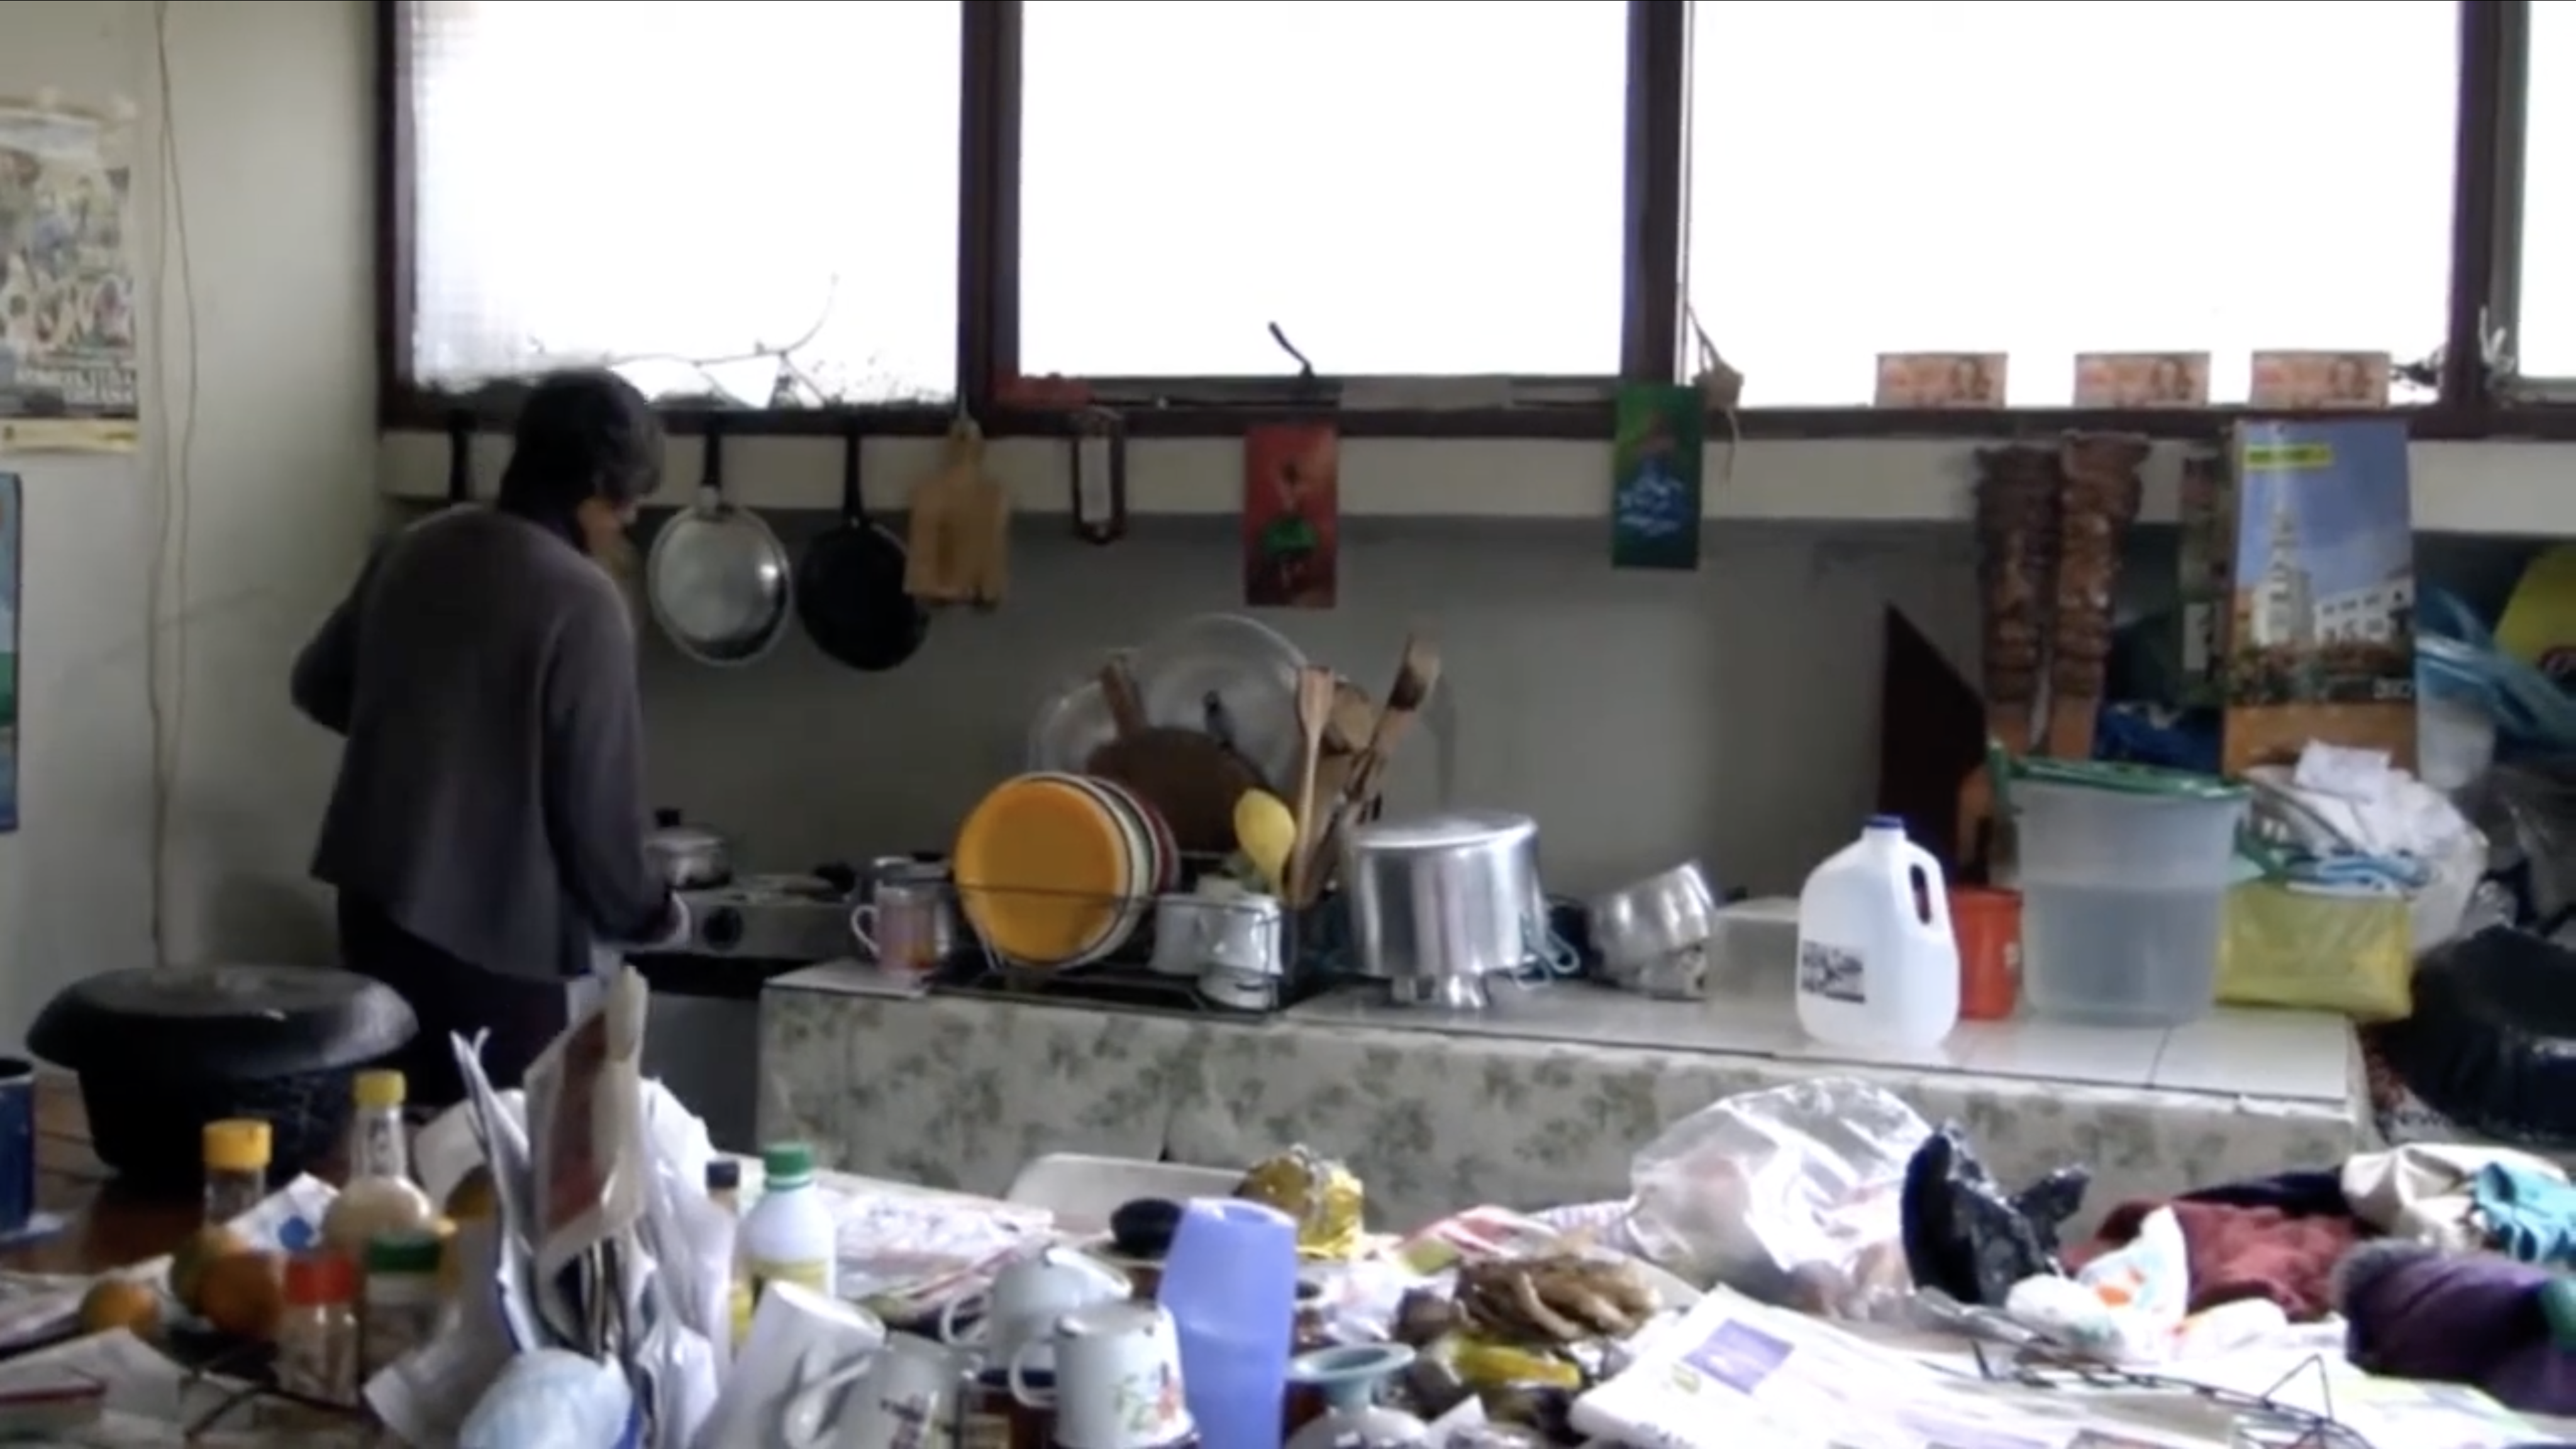
\includegraphics[width=\textwidth]{AlaDeriva_diaz2016_fotograma-00-34-25.png}
    \caption{AlaDeriva diaz2016 fotograma 00:34:25}
    \label{fig:AlaDeriva_diaz2016_fotograma_00_34_25}
\end{figure}

Cocina de tamaño medio, con una ventana grande que ocupa casi toda una pared. La luz natural entra por la ventana, creando sombras y contrastes en los objetos. Una persona de espaldas cocinando en una estufa. Una mesa grande cubierta de objetos, incluyendo platos sucios, bolsas, botellas y papeles. En las paredes hay cuadros y utensilios de cocina colgados. Una mesa en primer plano llena de objetos. La encimera al fondo está llena de utensilios de cocina. \parencite[fotograma: 00:34:25]{AlaDeriva_diaz2016}

\small
\begin{verbatim}
    graph TD
    A[[Anacronismo]]
    B[[Imagen-Síntoma]]

    A --> A1[Desorden flotante]
    A --> A2[Objetos sin tiempo, sin uso]
    A --> A3[Caos en silencio]

    B --> B1[Acumulación de objetos]
    B --> B2[Salud mental]
\end{verbatim}
\normalsize

\clearpage
\begin{figure}[h!]
    \centering
    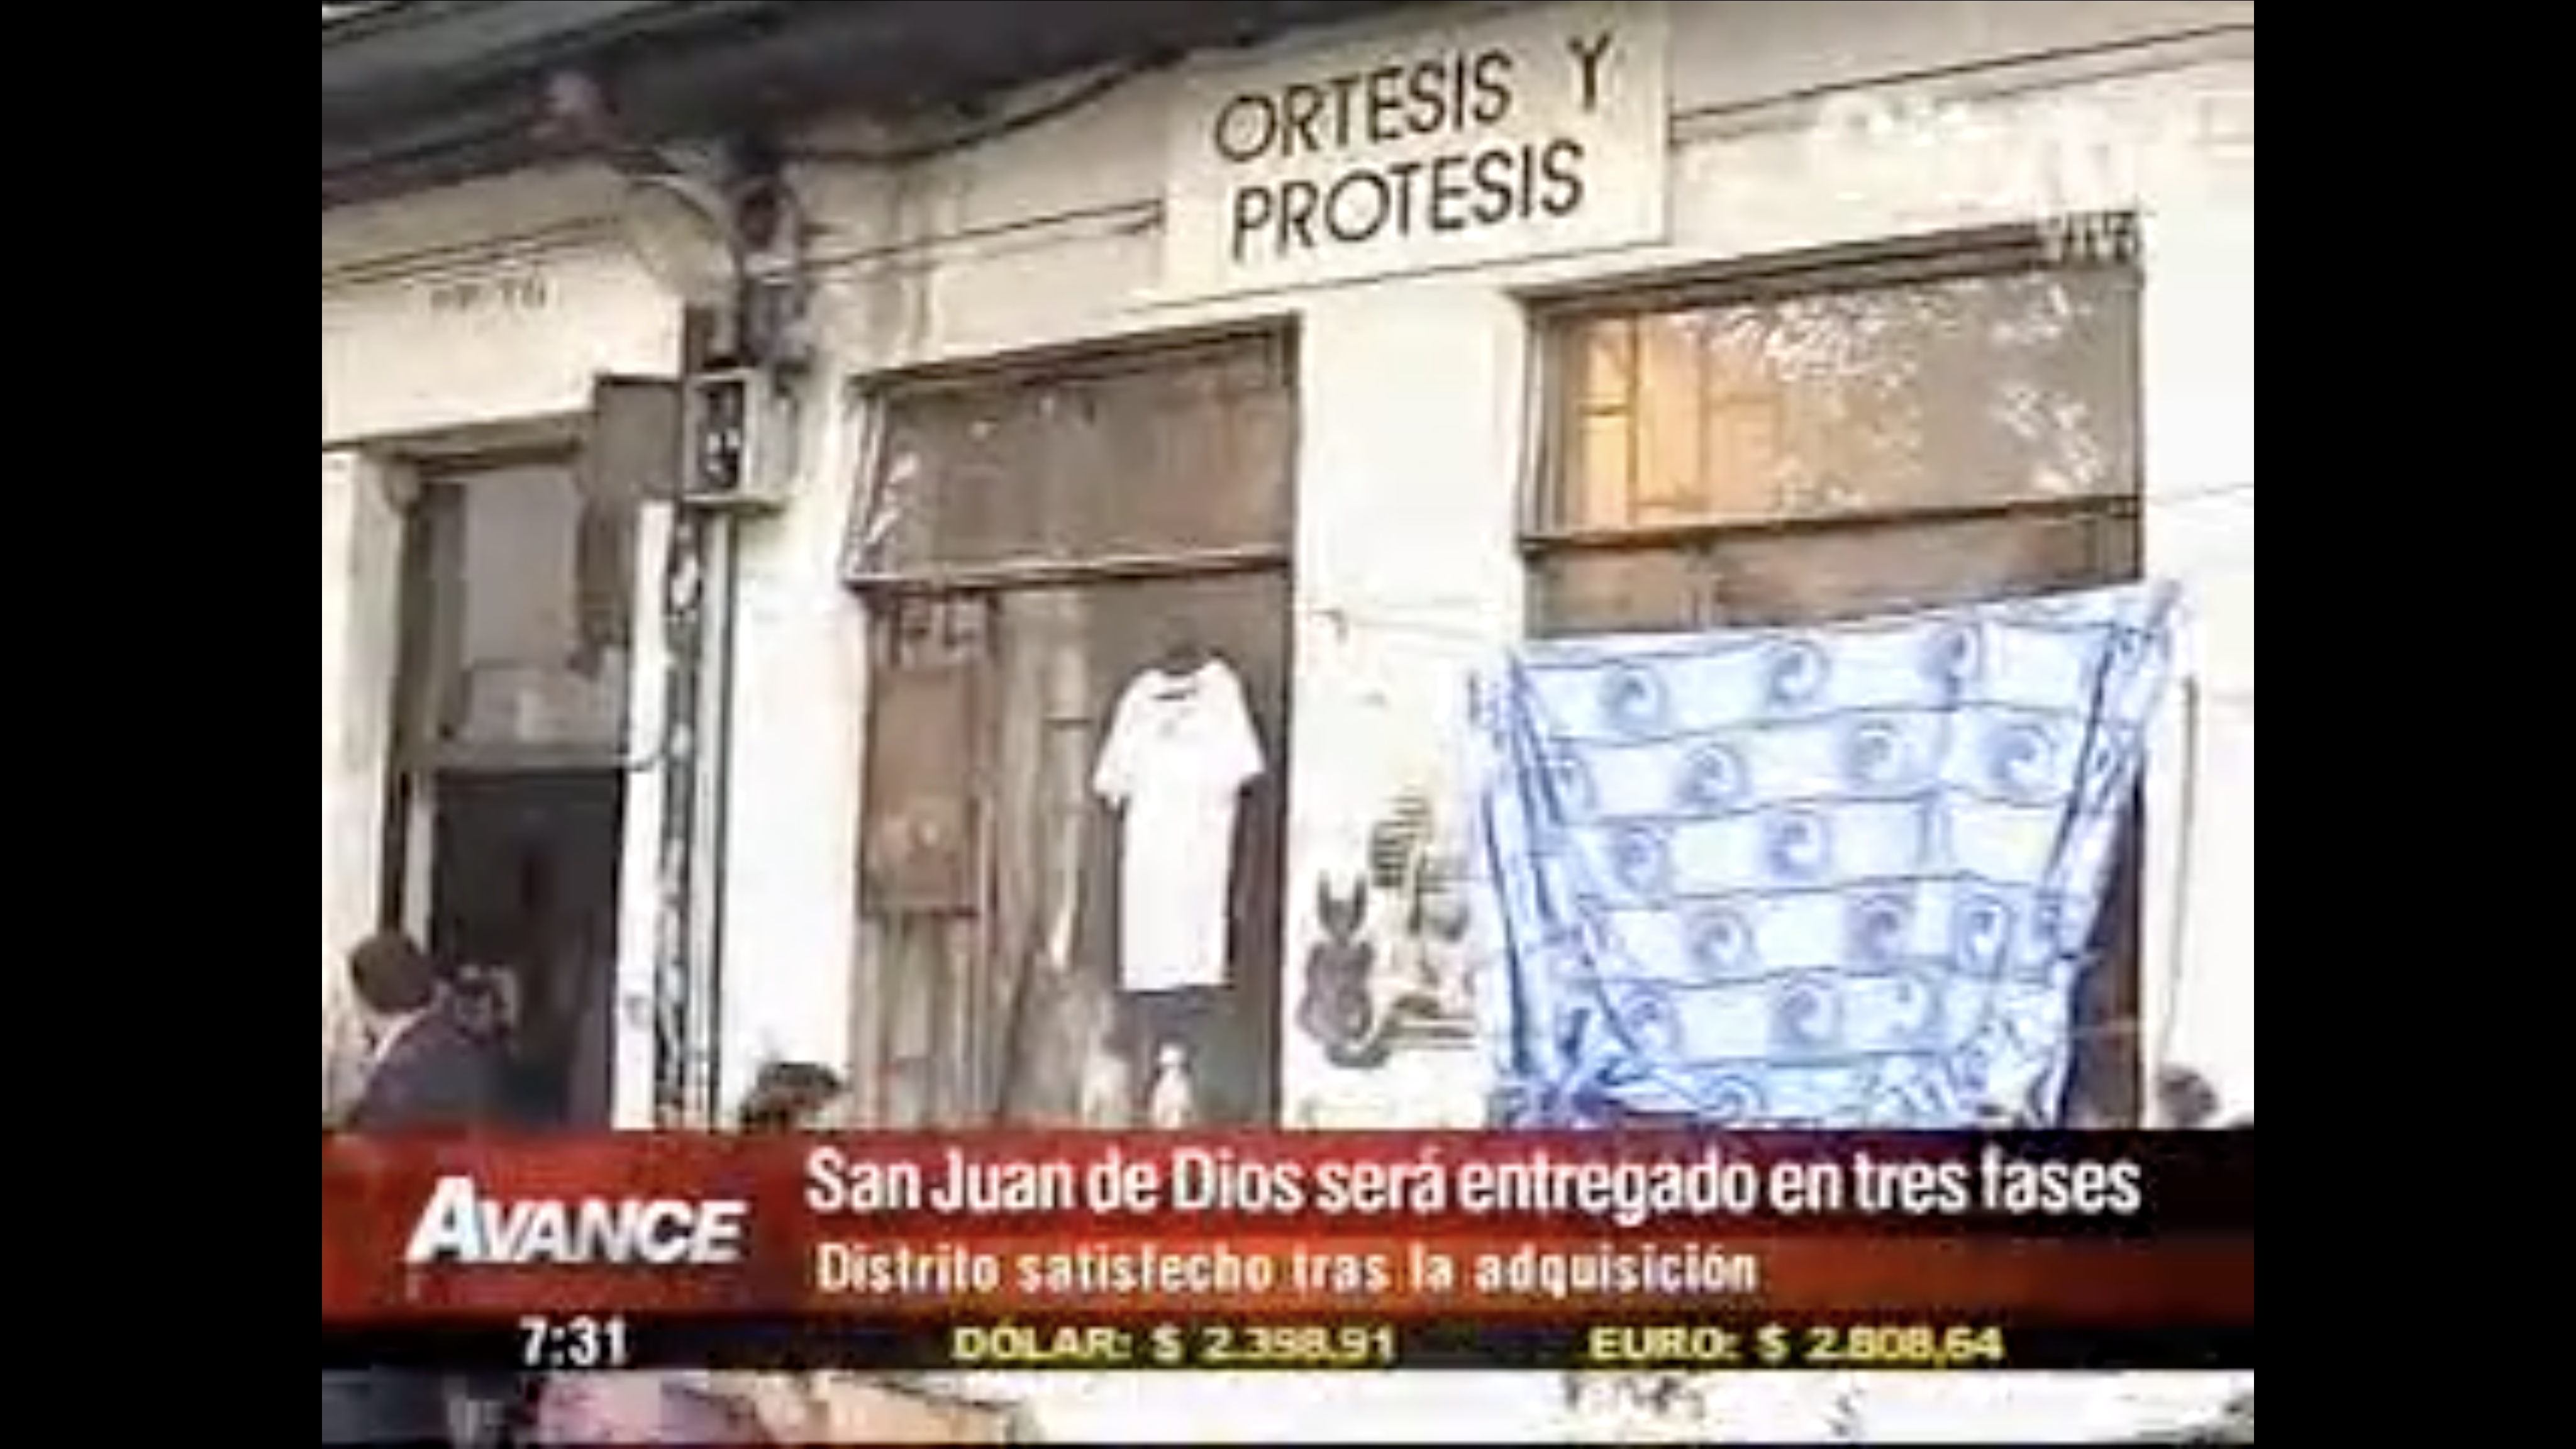
\includegraphics[width=\textwidth]{Citytv_junio2015_fotograma-00-00-16.png}
    \caption{Citytv junio2015 fotograma 00:00:16}
    \label{fig:Citytv_junio2015_fotograma_00_00_16}
\end{figure}

Fachada de un edificio con el letrero `ORTESIS Y PROTESIS'. Hay dos ventanas visibles: una parcialmente cubierta con plástico y una prenda blanca colgando, mientras que la otra tiene una tela clara con patrones color azul. Un cintillo de noticias rojo indica: "San Juan de Dios será entregado en tres fases" y "Distrito satisfecho tras la adquisición", mostrando además la hora 7:31 y los valores del dólar y el euro. Algunas personas aparecen parcialmente visibles en la esquina inferior izquierda. \parencite[fotograma: 00:00:16]{Citytv_junio2015}

\small
\begin{verbatim}
    graph TD
    A[[Anacronismo]]
    B[[Imagen-Síntoma]]
    
    A --> A1[Susurra historias de servicios olvidados]
    A --> A2[Arquitectura que deplora]
    A --> A3[Afirmaciones oficiales subyacentes]
    
    B --> B1[Exteriorización de hábitad humano]
    B --> B2[Contraste frase optimista y entorno desgastado]
\end{verbatim}
\normalsize

\clearpage
\begin{figure}[h!]
    \centering
    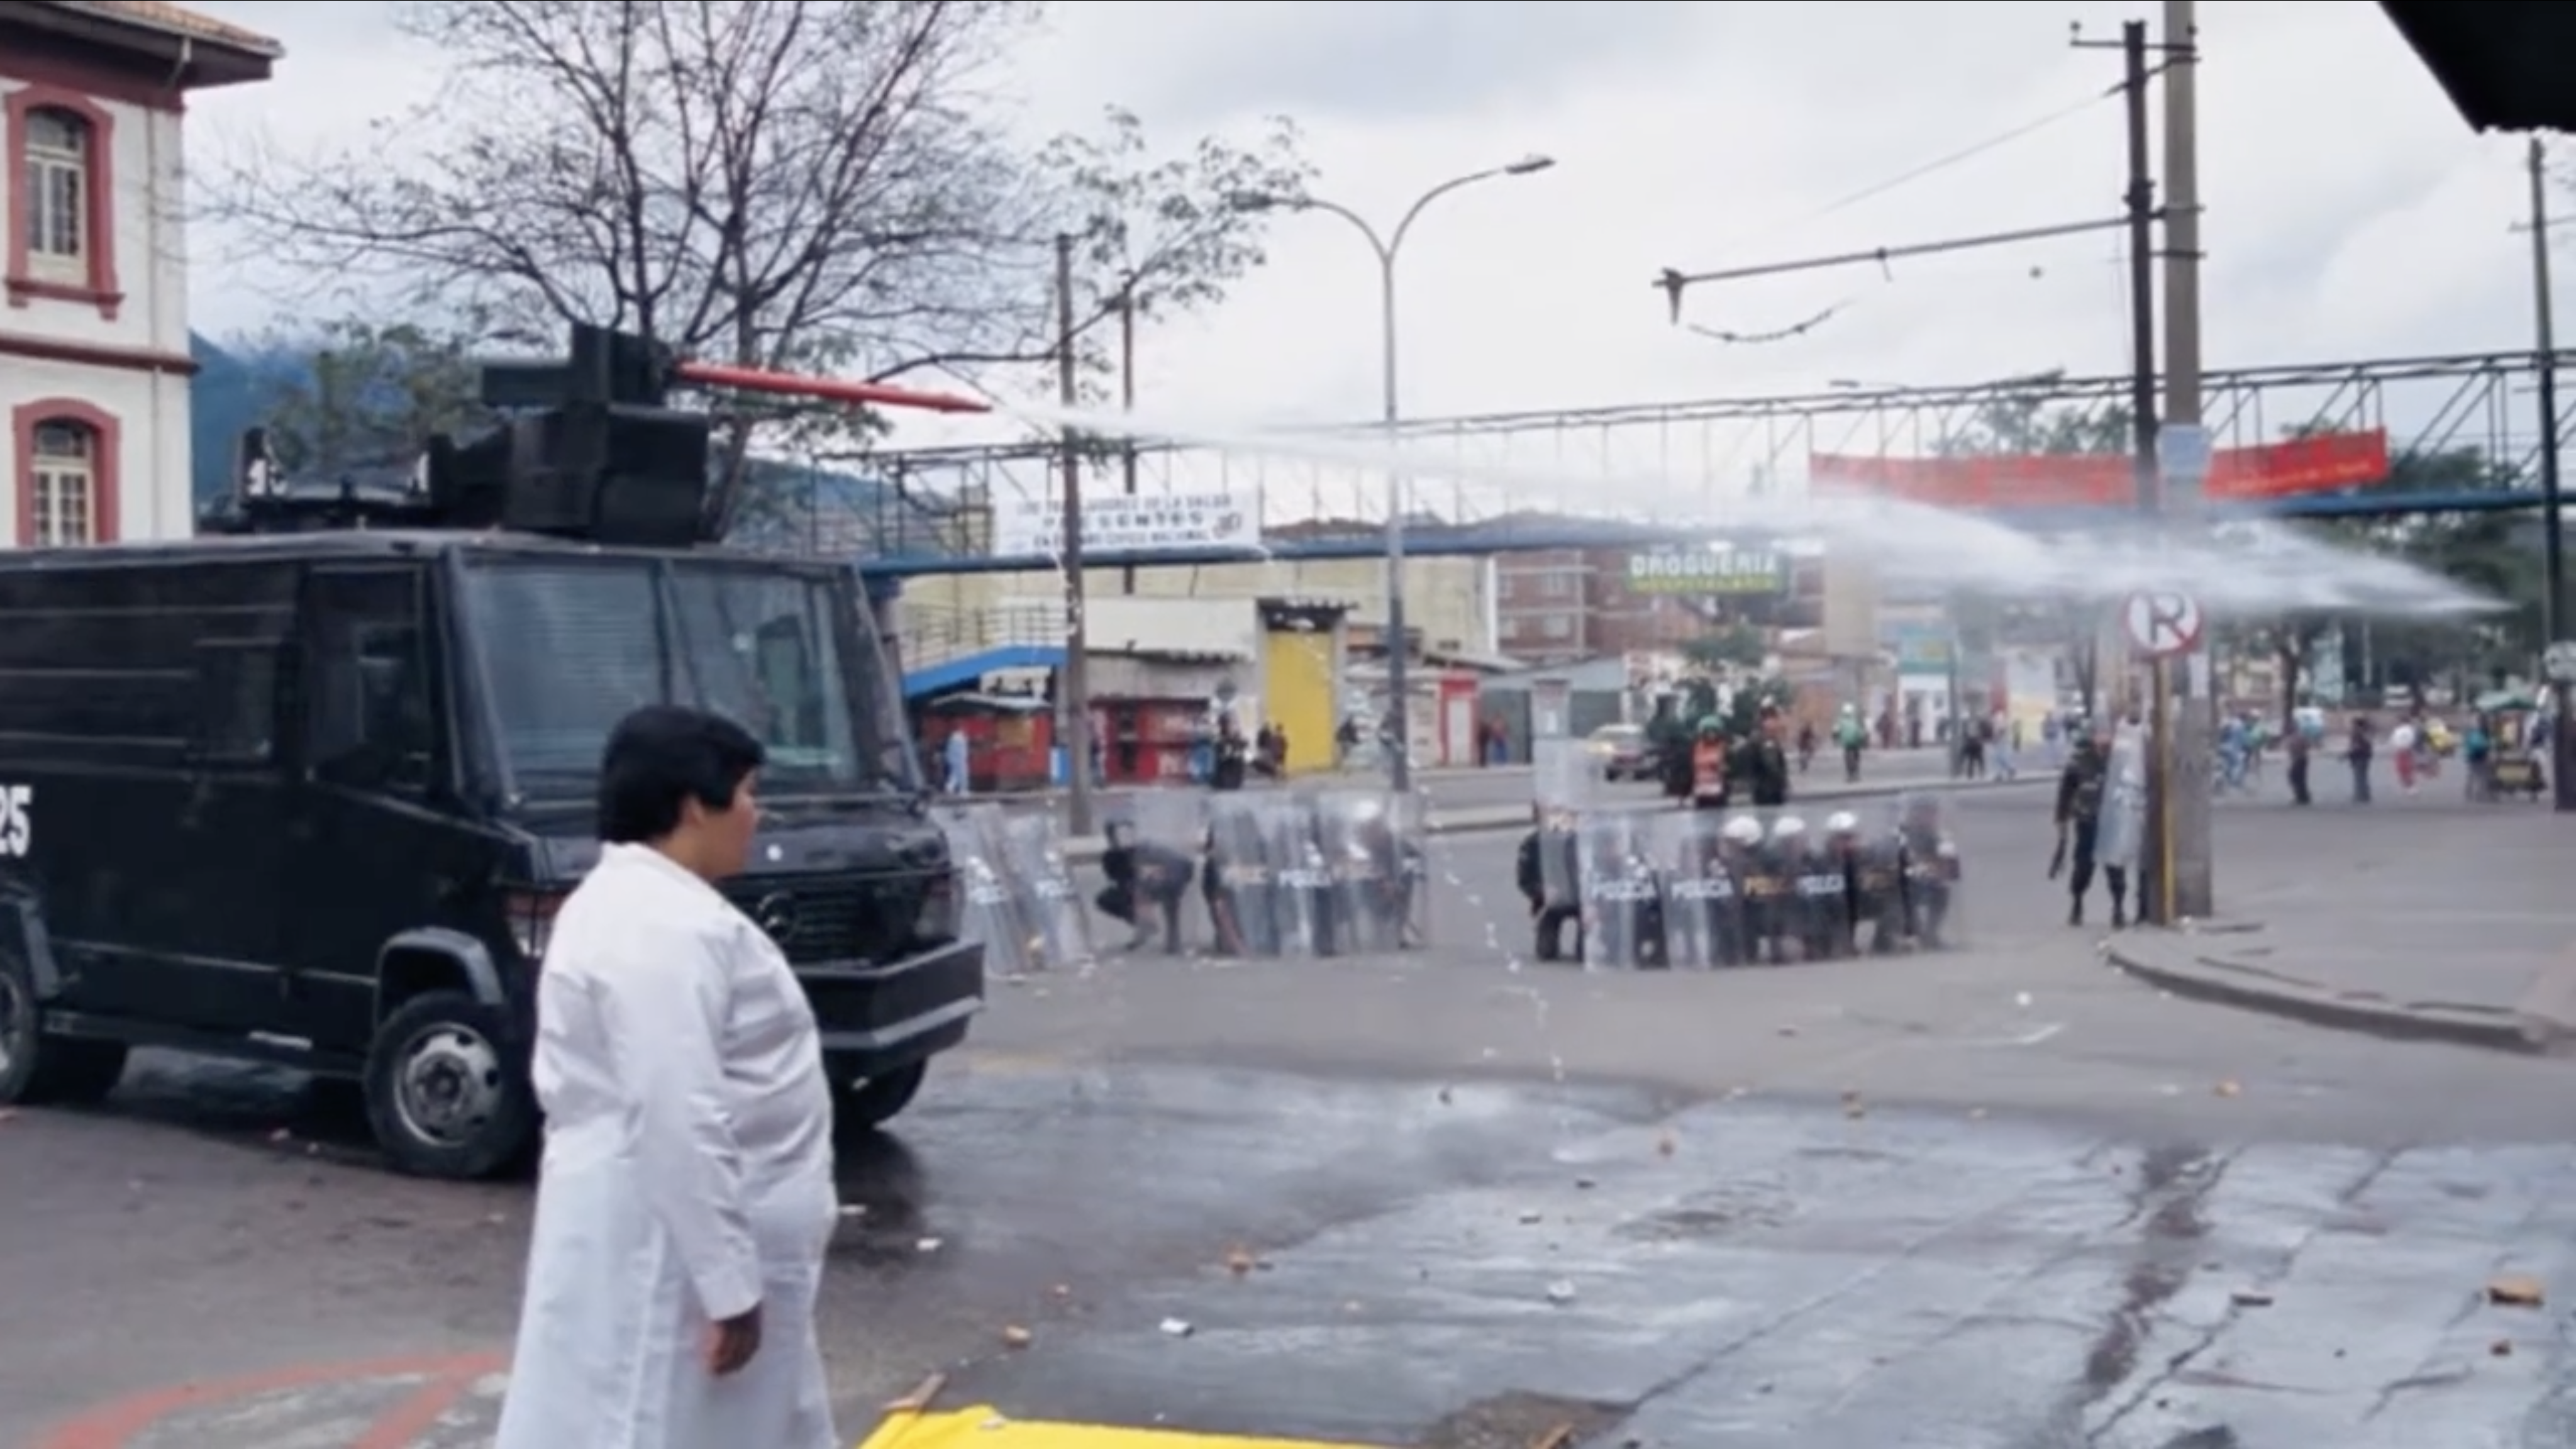
\includegraphics[width=\textwidth]{AlaDeriva_diaz2016_fotograma-00-05-54.png}
    \caption{AlaDeriva diaz2016 fotograma 00:05:54}
    \label{fig:AlaDeriva_diaz2016_fotograma_00_05_54}
\end{figure}

Exterior del HSJD carrera décima vista hacia el sur. Se observa un vehículo blindado negro tipo antimotines con equipo de dispersión de agua en el techo. En primer plano, sobre el pavimento mojado, hay una persona vestida con bata blanca. Al fondo se distingue un grupo de policías con escudos antidisturbios formando una línea, mientras un chorro de agua es disparado hacia la derecha de la escena. \parencite[fotograma: 00:05:54]{AlaDeriva_diaz2016}

\small
\begin{verbatim}
    graph TD
    A[[Anacronismo]]
    B[[Imagen-Síntoma]]

    A --> A1[Vehículo moderno en calle tradicional, coexistencia de épocas]
    A --> A2[Antidisturbios contra el cuidado]
    A --> A3[Tensión social latente]

    B --> B1[Desigualdad y control policial en sociedad]
    B --> B2[Disturbios como síntoma de descontento actual]
\end{verbatim}
\normalsize

\clearpage
\begin{figure}[h!]
    \centering
    \includegraphics[width=\textwidth]{archivoMargarita_6octubre2004.jpg}
    \caption{Archivo Margarita 6 de octubre 2004}
    \label{fig:archivoMargarita_6octubre2004}
\end{figure}

Sala de espera con una fila de asientos blancos de plástico montados sobre una estructura metálica negra. La pared es de color crema claro con algunos elementos montados como un tablero y un teléfono naranja. El piso tiene un patrón geométrico en tonos beige y gris. En la escena hay una persona vestida de negro que mira hacia el suelo a lo que perece ser un marco y cristal rotos. Hay una bicicleta, un balón de fútbol y detrás de la hilera de sillas a la izquierda una puerta con letreros de `SELLADO'.

\small
\begin{verbatim}
graph TD
    A[[Anacronismo]]
    B[[Imagen-Síntoma]]
    
    A --> A1[Sala de espera vacía y austera]
    A --> A2[En tonos apagados]
    B --> A3[Lo lúdico se asoma]
    
    B --> B1[Soledad y aislamiento del individuo]
    B --> B2[Deshumanización en espacios institucionales]
\end{verbatim}
\normalsize

\clearpage
\begin{figure}[h!]
    \centering
    \includegraphics[width=\textwidth]{archivoJuanArroyo_10September2022_04_33.jpg}
    \caption{Archivo Juan Arroyo 10 de Septiembre 2022}
    \label{fig:archivoJuanArroyo_10September2022_04_33}
\end{figure}

\textit{Performance}. La imagen muestra edificio San Lucas en proceso de renovación o reparación. En la primera fotografía, se observan dos personas realizando tareas en el espacio - una sentada en el suelo trabajando con herramientas, y otra de pie observando. La segunda fotografía muestra a una persona sola de espaldas en el mismo espacio, se aprecia ropa colgada en una cuerda, dando la impresión de un espacio doméstico improvisado. Las paredes desgastadas, ventanas en crudo y suelo de concreto sugieren que el edificio está en una fase inacabada o de transición. Se yuxtaponen  escenas cotidianas de trabajo y vida dentro del entorno hospitalario.

\small
\begin{verbatim}
graph TD
    A[[Anacronismo]]
    B[[Imagen-síntoma]]

    A --> A1[San Lucas cambia]
    A --> A2[Ropa al viento susurra]
    A --> A3[Hogar casual]

    B --> B1[Personas habitando en contexto disruptivo]
    B --> B2[Ningún mobiliario]
\end{verbatim}
\normalsize

\clearpage
\begin{figure}[h!]
    \centering
    \includegraphics[width=\textwidth]{2011 Nicolas Van Hemelryck - San Juan sin Dios055.jpg}
    \caption{2011 Nicolas Van Hemelryck - San Juan sin Dios - 055}
    \label{fig:2011NicolasVanHemelryckSanJuansinDios-055}
\end{figure}

Sala de cirugía, interior deteriorado, ventanales que dejan entrar luz natural, contrastando con lámparas eléctricas colgantes. En este espacio se observan personas sentados en el piso sobre colchonetas y frazadas, rodeados de ropa y objetos personales. La escena revela síntomas de de usos disruptivos de ambiente para el cuidado quirúrjico y en hábitat doméstico. Foto del libro \parencite{Hemelryck2011}

\small
\begin{verbatim}
    graph TD
    A[[Anacronismo]]
    B[[Imagen-Síntoma]]

    A --> A1[Ventanas de otra era iluminan penumbras del presente]
    A --> A2[Despojos textiles de tiempos mezclados yacen inertes]
    A --> A3[Sombras del pasado acechan en la quietud actual]

    B --> B1[Abandono y precariedad se cuelan por los muros]
    B --> B2[Niñez expectante aguarda en silencio un futuro incierto]

\end{verbatim}
\normalsize


\clearpage
\begin{figure}[h!]
    \centering
    \includegraphics[width=\textwidth]{Ahumada2013_cuadro1.png}
    \caption{Cuadro I. Juan Camilo Ahumada, Tiempo de dios. 2013}
    \label{fig:Ahumada2013_cuadro1}
\end{figure}

\parencite[p. 10]{Ahumada2013}

\small
\begin{verbatim}
graph TD
    A[[Anacronismo]]
    B[[Imagen-Síntoma]]
    
    A --> A1[Impecabilidad atemporal y vacío]
    A --> A2[Guantes quirúrgicos y el aliento]

    B --> B1[Desconexión y falta de propósito]
    B --> B2[Automatización existencial]

\end{verbatim}
\normalsize

\clearpage
\begin{figure}[h!]
    \centering
    \includegraphics[width=\textwidth]{Ahumada2013_cuadro4.png}
    \caption{Cuadro IV. Juan Camilo Ahumada, Tiempo de dios. 2013}
    \label{fig:Ahumada2013_cuadro4}
\end{figure}

\parencite[p. 12]{Ahumada2013}

\small
\begin{verbatim}
    graph TD
    A[[Anacronismo]]
    B[[Imagen-Síntoma]]
    
    A --> A1[El doctor, un niño que no habla, cirugía moderna]
    A --> A2[Bata blanca y tecnología]
    A --> A3[La humanidad interna revelada]
    
    B --> B1[Avances médicos y fragilidad del cuerpo]
    B --> B2[Ética y cuidado humano]

\end{verbatim}
\normalsize


\clearpage
\begin{figure}[h!]
    \centering
    \includegraphics[width=\textwidth]{Una de las resistencias Karina Moreno 2015_5.jpg}
    \caption{\textit{Una de las resistencias} Ana Karina Moreno, 2015.}
    \label{fig:KarinaMoreno2015}
\end{figure}

Interior de edificio, postes de madera sosteniendo el techo sobre batas blancas y verdes apiladas. La tela se ve usada y pulcra, con arrugas y pliegues naturales.

\small
\begin{verbatim}
    graph TD
    A[[Anacronismo]]
    B[[Imagen-Síntoma]]
    
    A --> A1[Anhelo atemporal de pureza ]
    A --> A2[Contraste tela y rudeza natural]
    A --> A3[Ropa y pilar]

    B --> B1[Resistencia y fragilidad]

\end{verbatim}
\normalsize


\clearpage
\begin{figure}[h!]
    \centering
    \includegraphics[width=\textwidth]{Duarte_didacticos.jpg}
    \caption{Didácticos para una sala de espera, Jenniffer Duarte 2015}
    \label{fig:JennifferDuarte2015}
\end{figure}

Colección de cubos apilados de madera, cada uno pintado con una letra del alfabeto y una ilustración en blanco y negro de diversos animales y partes del cuerpo humano, como cerebros y pulmones, en un estilo gráfico similar a grabados médicos antiguos. Sobres con hojas de historia clínica.

\small
\begin{verbatim}
    graph TD
    A[[Anacronismo]]
    B[[Imagen-Síntoma]]

    A --> A1[Bloques de juguete y grabados de ciencia]
    A --> A2[Lúdico infantil y la anatomía clásica]
    A --> A3[Fascinación perenne por el cuerpo]

    B --> B1[Alfabetización visual y biología humana]
    B --> B2[Curiosidad y asombro]
\end{verbatim}
\normalsize

\clearpage
\begin{figure}[h!]
    \centering
    \includegraphics[width=\textwidth]{si no hay justicia hay performance.jpg}
    \caption{2016 Luisa Fernanda Vela - Al margen}
    \label{fig:LuisaVela2016}
\end{figure}

El montaje fotográfico yuxtapone dos retratos en blanco y negro de mujeres jóvenes de épocas distintas. A la izquierda, una imagen antigua muestra una mujer con peinado y ropa de los años 50, mirando pensativa con un dedo en los labios. A la derecha, una imagen contemporánea presenta una mujer con uniforme de enfermera y gesto serio, con la mano en la barbilla en actitud reflexiva. Debajo, un texto en español conecta ambas imágenes: ``Si no hay justicia, hay performance''.

\small
\begin{verbatim}
    graph TD
    A[[Anacronismo]]
    B[[Imagen-Síntoma]]

    A --> A1[Moda y peinados de distintas décadas se encuentran]
    A --> A2[Actitud contemplativa perdura a través del tiempo]
    A --> A3[Anhelo de justicia late en poses de mujeres pensativas]

    B --> B1[Mujeres en roles tradicionales cuestionan su realidad]
    B --> B2[Gesto meditativo surge ante injusticias presentes]
\end{verbatim}
\normalsize

\chapter{Escenificación: montaje de imágenes}
\section{Conclusiones}

El montaje permite escenificar la emergencia de temporalidades, enunciaciones, anacronismos y otros síntomas en el conjunto de registros artísticos, imágenes documentales y textos visuales. A través de este proceso, se revela el entramado de atemporalidades y se genera una experiencia de sentido mediante los pasajes simbólicos del caso de estudio. El montaje constituye, entonces, un análisis interpretativo sobre la selección de imágenes que expresa espacial y temporalmente en <<cuadros>> el entramado visual y social, creando un ambiente de interpretación exploratoria que deriva en experiencias de construcción de sentido.

Denominamos escenificación tanto a la experiencia como al resultado del montaje utilizando las imágenes seleccionadas. El ordenamiento de las escenas representa una forma espacial de montaje que permite unir lo comprensible con lo imaginario, generando experiencias de sentido que confrontan nuestra mirada con el entramado sistémico de esta compleja situación social.

Las escenas materializan la intersección conceptual entre la antropología de la imagen y el método socio semiótico. La experiencia de inmersión en el recorrido visual sobre el San Juan de Dios ofrece posibilidades interpretativas que impulsan el deseo de comprensión, guiando al observador hacia la revelación de los entramados emergentes en este discurso no textual. Se omite deliberadamente el enfoque historicista, pues el objetivo es resaltar la existencia del anacronismo sin necesidad de una enunciación secuencial de acontecimientos.

El fenómeno sociocomunicativo del caso de estudio se manifiesta a través de elementos anacrónicos que atraviesan la imagen no-domesticada - aquella que se desprende de propósitos publicitarios o periodísticos - y se integra en redes dialógicas no-textuales mediante el montaje con otros discursos visuales. Esta interacción facilita la emergencia de la imagen-síntoma y los indicios de anacronismos.

La metodología propuesta permitió materializar objetos mediales para la conceptualización. El ``juego'' con las imágenes funcionó como estrategia de trabajo para abordar ideas abstractas, asociarlas y organizarlas espacialmente.

El montaje intencionado para la construcción de sentido enfatiza los síntomas visuales del discurso, generando conjuntos y redes significantes e imaginarias, interpretables desde los fundamentos conceptuales de la antropología de la imagen y la socio semiótica. Estas redes significantes o "fascinaciones" de la mirada subrayan la atracción irresistible del observador, quien en su gesto de registro o creación de imagen materializa enunciaciones emocionales y de sentido.

Un aspecto recurrente es el encuadre de lugares y objetos deteriorados por el tiempo: las imágenes evidencian el triunfo del agua, el musgo y la hierba sobre las superficies. Esta característica visible contrasta con el impulso de quienes han resistido y cuidado el San Juan, personas que han luchado a contracorriente mediante actos de expresión visualmente documentados, generando impulsos de resistencia ante la hostilidad del contexto y las circunstancias.


\addtocontents{toc}{\vskip10pt\hfill\textbf{|}\hfill\vskip10pt}

\clearpage
\listoffigures
\listoftables   

\phantomsection
\printbibliography[title={Bibliografía}, nottype=online]

\phantomsection
\printbibliography[title={Videografía}, type=online]

\addtocontents{toc}{\vskip10pt\hfill\textbf{|}\hfill\vskip10pt}

\footnotesize
\appendix
\chapter{Apéndice - Entrevista a Juan Camilo Ahumada}
\label{apendiceA}
Juan Camilo Ahumada
Juan Carlos Arroyo

Entonces te acabo de contar, sé que en el 2013 tu hiciste este… o por lo menos se publicó digamos.

Ahumada: Sí, eso.

Se publicó el guion, y en el 2016 hubo un performance, y en el marco digamos de esta exposición, el distrito hizo un evento con respecto a Arte y paz, y ahí digamos en el marco de esto David Lozano, que es un maestro en artes plásticas fue de la Nacho, hizo otro performance y entonces como que este es mi corpus de investigación.

Chévere, pues digo chévere estar como en la periferia de esas cosas, pues yo no… aunque trabajo en torno a los referentes concretos visuales, musicales pues de corte estético, y también unos referentes teóricos obviamente pues al afrontar como un ejercicio creativo, en este caso los referentes eran cosas muy, muy, muy distantes al hospital, porque era una cosa que era de alguna manera una premisa cuando yo arranqué, yo quería hacer algo a unos testimonios, primero vi la cosa es así. Me disculpa ser tan escueto, pero este es el proceso de creación, yo vi unos videos en YouTube sobre el hospital San Juan de Dios, obviamente como inquieto por hacer algo en torno al hospital San Juan de Dios y como tratando de indagar en quienes habitaban el lugar, porque lo que más me interesaba bajo este tiempo en el que estuvo cerrado, y algunas personas decidieron irse a vivir allá. La obra gira en torno a eso, básicamente entre lo que pasaba entre estas personas ahí adentro, e hicieron un intento de documental que colgaron en YouTube que está en acabado, estoy hablando como en el 2005 tal vez, finales del 2008 no se, por ahí antes del 2009 en todo caso.
Y luego me surgió la posibilidad de hacer una residencia artística en Buenos Aires, con un maestro de escritura gramática que se llama Alejandro Tantanian, y cuando yo llegué a Buenos Aires llevaba todos los materiales, todos los testimonios, y una suerte como de caprichos estéticos.

¿Y esos testimonios como los recogiste? 

Tenemos los del video.

a los del video ok.

Luego yo tuve la oportunidad de conocer una señora que se llama Teresa Díaz, que lideraba en ese momento, yo no sé ni siquiera si la señora está viva porque no tuvimos ninguna relación, nos vimos una vez charlamos y ya, yo la grabe en video. Y pues ella estaba como muy interesada en hablar como del movimiento político que se había ido gestando ahí, el ejercicio de resistencia civil y esas cosas, pero yo la sentía como decirlo, como muy en el terreno de lo político.

Si.

Yo quería cuestionar la cosa desde otros niveles. También porque a nivel de lo político eso estaba completamente sesgado entre buenos y malos, y los buenos son los que están ahí y los malos son los que los quieren sacar, como en la estrategia del caracol y no es así, la cosa pensarla de esa manera sería aplanar de alguna manera el conflicto, yo sentía que ya estaba aplanando el problema definiéndolos entre buenos y malos, pero de ella pude coger como una suerte de voz, y una suerte de melancolía en el ejercicio de habitar este lugar y todo esto se articulaba a la perfección como con una cosa que yo quería tratar de materializar que era como unos universos de la desesperanza, y en ese momento este texto surge con otros dos, es decir como en el mismo momento y por la misma inquietud con otros dos que son absolutamente diferentes, uno que se llama llenasvenbrandy y el otro texto que se llama noche de alacranes, que son también como unas obras que tratan de darle vuelta a esto de la des-absoluta esperanza, como de la condición humana en ese momento del ocaso de la vida, como de esperar la muerte, como que la única posibilidad de esperar sería esperar morirse y entretenerse durante la vida, como sin ningún oficio concreto bueno… y esta obra se ganó el premio distrital de dramaturgia y entonces logro como sacar la cabeza por ese trio de obras, pero igual las otras están ahí, llenasvenbrandy la montamos y era como de alguna manera la preocupación que tenía por la desesperanza, partiendo de la desesperanza llegaron los testimonios del San Juan de Dios, y hablándole a unos amigos de este proyecto que yo tenía, alguien me dijo que conocía quien dirigía el movimiento pues de las personas que habitaban allí, que era doña Teresa Díaz yo me reuní con ella, y con estos testimonios me fui yo quería también hacer algo entorno como a lo trágico, pensando en términos teatrales, es decir quería hacer algo que estructuralmente se pudiera definir dentro de lo que es la tragedia en el teatro. Y para eso entonces me apoye de una ópera que es este kindertoten líder, que son las canciones de los niños muertos, the mahler, había otro referente ahí bien importante que ahora no lo recuerdo. Bueno pero había otro referente de corte musical, y tratando un poco como de… esos son los insumos concretos digamos las materias con las que trabaje, ahora mi aporte pues gira en torno al tratar de construir dos universos ahí entramos hablar de la obra, yo creo que la obra se sostiene como en dos universos, uno que son las cosas que suceden al interior de las personas, como el terreno del pensamiento, de la evocación, o del recuerdo bueno en fin, las cosas que les pasan por dentro a las personas, y otro plano que se contrasta como de una manera medio abrupta también ahí en la obra es lo cotidiano, y de alguna manera es como lo ordinario, el orden normal de las cosas de alguna manera lo vulgar, lo escueto, trivial si se quiere la lógica de la cotidianidad de una manera más… es que la palabra no es costumbrismo, pero la cosa si es como de una forma mucho más concreta, las cosas concretas los panes, las mesas, los dados, las cosas concretas de la vida de estas personas, y en el texto trato de armar. Originalmente este texto puede que esto de luces, originalmente el texto se llamó viacrucis y era una idea de hacer las estaciones, la idea digamos como estaba pensado era como unas estaciones en el espacio y que los espectadores pudieran transitar el espacio viendo estas situaciones instaladas en diferentes lugares, entonces hay una estructura narrativa que no es lineal y que se sostiene como en la construcción de estos pequeños universos que son casi que independientes. Y estructuralmente pues el recorrido quedo así como si arrancara, como una suerte de vocación, en la mitad está toda esta tensión con la cotidianidad, con el mundo concreto y terminamos como tratando de romper esta idea de la esperanza cristiana y del tiempo de Dios.
Ayer un muchacho en el bus, un ex drogadicto mencionaba el capítulo y el versículo de Ezequiel 3:3 que dice que los tiempos de Dios son perfectos y que todo tiene lugar y tiempo en el mundo de Dios y bueno estas cosas, que era de alguna manera como la justificación que ellos me daban o que yo sentía de ellos y es que el tiempo de Dios es perfecto y esto va a durar lo que Dios quiera de alguna manera, porque también hay que decirlo esto sucedió antes del gobierno Petro, cuando premiaron esta obra que fue en la mitad del gobierno Petro el problema se estaba disolviendo es decir si ese texto no lo publican en ese momento pierde completa vigencia, aunque la relación ahí no ha sido asumida tan directamente digo como por la gente que lee y eso.

No pero tiene mucho sentido es decir por ejemplo para mí sería muy difícil no reconocer digamos el momento en que estas obras fueron publicadas.

Si tiene mucho que ver con eso, claro

Hay algo de mis hipótesis pero tiene que ver con que el discurso digamos político social encuentra ahí un fenómeno en donde confluyen muchos de los discursos que de una manera a quienes estaban metidos en la problemática les servía el discurso político, se prestan mutuamente los intereses.

Si como un terreno fértil no.

Si.

Un terreno fértil como para que todos de ahí saquemos una buena cosecha seguramente fue así, porque también el momento en el que yo estaba en estas, estaba dándose esto con el gobierno Petro, como las discusiones, las conversaciones, la posibilidad de negociar el predio con la gobernación de Cundinamarca y esto, y un poco como se veía de lejos, porque yo pude ver además desde Buenos Aires como se veía de lejos la cosa, era pues si estamos abonando el terreno y ya luego todos, además todos incluso el gobernador de Cundinamarca que en ese momento era un hampón, todos sacaremos provecho.
Y ya el ejercicio literario pues fue un poco darme la pelea por lograr ser un poco coherente en la construcción de estos universos, y el texto está construido por unos hilos como narrativos que tratan de vincular los diferentes fenómenos. Pero si quiere hablemos de las escenas sí.

Por favor.

Ya hablando de eso de las escenas que cada una tiene un universo independiente, pues este primer cuadro que es solamente una acción, que este niño que está inflando unos guantes y está dejándolos pasar tenía un poco… se lo voy hablar desde la intención literaria de la teatral.
En lo literario yo quería como de alguna manera instaurar un tono para el texto, una manera de escritura, una textura para el texto de alguna manera como abriéndole la puerta al espectador hacia la manera en la que yo quería narrar la  historia, y creo que teatralmente espacialmente esto nos permitía como construir una metáfora del paso del tiempo, en ese momento una premisa era como una apertura hacia la eternidad, como hacia algo que no tuviera fin, bueno en fin, y esta figura del niño que va acompañando todas las historias o que las va atravesando pues de alguna manera era como presentar el anfitrión que va a ir con la gente haciendo el recorrido, pensándolo así digamos.

Si.

Este segundo cuadro que es el de Rosalía, es la presentación de este personaje, Rosalía es un personaje real que habitó con ellos en el hospital y que efectivamente la mandaron a habitar al edificio psiquiátrico, y que además es un personaje bellísimo, yo no tengo ningún vínculo personal con ninguno de ellos, pero si tuviera que tenerlo preferiría tenerlo con Rosalía, porque a pesar de que tiene una distorsión del pensamiento y que piensa de una manera paralela digamos a la convencional, me parece una mujer de una sensibilidad absolutamente particular y era la única digamos que estaba… voy a decirle el gesto y usted hace la interpretación, cultivaba y tenía animales dentro del lugar y se había dado una pela muy grande porque le respetaran el patiecito donde tenía sus matas y cultivaba, es decir no solamente matas sino cultivaba cosas y cuidaba unos animales pollos, perros bueno en fin, y ahí yo vi como un gesto más de empoderamiento como muchísimo más agresivo y eso le significó estar alejada de  los demás, de todos los demás que estaban habitando el Hospital, y además estaban en una pelea constante con todos muy fuerte. pero Rosalía también tenía un hijo, que es un hijo que luego se va a convertir aquí en el invalido un hijo con una discapacidad que yo nunca conocí, al que siempre me mencionaron y que siempre tuve ahí como en un ideal medio macabro de un muchacho quieto dentro de una pieza o dentro de un consultorio convertido en pieza, estático mirando una pared, contando ladrillos en una pared sin posibilidad de moverse ni de prender un televisor, ni de escuchar radio, ni de hacer nada en su vida más que ver y contar los ladrillos de una pared.
Bueno pero entonces aquí básicamente la presentación de este personaje, y tratar de ir instaurando el lugar, porque ella arranca como contando… describiendo quienes habitaban unos consultorios de consultas en un primer pasillo.

Este tercer cuadro es la presentación de Teresa Díaz, a quien le adjudicó el hijo de Rosalía, si es decir el hijo de la vida real de Rosalía yo se lo pongo a Teresa Díaz y la pongo como en un juego hay de amor y odio con el hijo en esta figura que tal vez está más adelante, hay una imagen en la que ella está afeitando al hijo acá, afeitar al hijo es cuidarlo, acariciarlo y también querer acabar con su vida que era un poco como esta cosa como tratar de construir esta imagen de la mamá que tiene que afeitar al niño inválido pero que en algún momento piensa jalar la cuchilla y dejar ahí, dejar ahí pues.
Esta es la presentación entonces de la enfermedad del muchacho, y aquí vuelve el niño y esta lógica como de la práctica científica y destacas en las que ellos fueron tan diestros de la… como de la  concreción de su oficio que tenía que ver con sangre, manipular carne, mover viseras, ajustar compresas llenas de sangre, botar restos de seres humanos estas cosas, aquí trataba de metaforizar por medio de un juego de un niño que es cirujano y que trata de abrir dentro de un muñeco y tratar partes y sacar partes dentro del muñeco mientras eso es amplificado en una proyección, de alguna manera quería que esto, la imagen que yo tenía era como de una cirugía que estaba sucediendo adentro y que se podía ver proyectada en el hospital como si quitaran partes digamos del espacio y adentro encontraron partes humanas, de alguna manera como una vuelta ahí a la imagen que era una imagen de referente con la que yo me había sido de un niño rompiendo un muñeco con un bisturí, trate de componer esa… además de esta imagen salió este niño que era vuelvo y digo el elemento que nos atravesaba como anfitrión, como se llama el Aqueronte que va con uno atravesando pues haciendo el recorrido como anfitrión.

Pero dices del hospital arquitectónicamente?

Si. Espacialmente, y además esto es una cosa que luego se volvió bien difícil, y es que yo escribí esto para ese espacio, pensando en ese espacio y nunca, nunca pude ni siquiera pensar en un proyecto creativo que tuviera que ver con eso y tuve que quedar satisfecho.

Pero recorriste ese lugar, digamos físicamente?

Sí, es decir está y hay una de las escenas que es esta donde están con el padre y que están haciendo como unas oraciones, está la del animero, es un recorrido por un espacio real y yo trato de darme la pela por describirlo, aunque pues es que yo soy muy mal autor entonces no lo logró describir a cabalidad, pero la idea si es que aquí quede el espacio todo esto del ritual del rezo y tal, aquí entre nos pues digamos es una manera de construir el espacio, y es una manera además densa y aburrida porque esto estructuralmente supone un momento que la obra pare como después de ir en quinta, mandar a primera de una y que toca haga como… y vuelva a instaurarse en otro ritmo muchísimo más lento.

Ya.

Que es un problema digamos para el ritmo de la obra, pero era necesario porque yo quería el recorrido espacial, es decir quería la gente en una procesión con esta lógica además del animero paisa que no se si conoce esta historia del animero, de un tipo que quería tal cual un poco como animero coro de actores haciendo de almas y espectadores transitando la representación.

Guiados por ese animero.

Si, si y construyendo el espacio a partir de eso, y había otro referente importante en esas tres obras además, yo creo que también un poco en mi manera de escribir y mi manera de articular las historias o de contarlas y es la cultura popular, obviamente distanciado del teatro popular y esas cosas que no tienen nada que ver con esto, pero si quería un poco tratar de también cuestionar esto desde la cultura popular, es decir esto como se pensaría también la nostalgia si el único referente posible fuera Alci Acosta.

Aja ok.

Si como ponerles palabras al dolor si el único referente es Vicente Fernández, por decirlo de alguna manera, o Roberto Carlos que aparece acá tratando de escribir una relación amorosa con un tipo que solamente escucha Roberto Carlos que es un personaje muy indo.
Y ahí empiezan aparecer este tipo de cosas, por ejemplo como esta escena es la escena número cinco de Edelmira, en la que hay como una suerte de rezo en la que ella está sola, en un espacio como con unas imágenes sagradas, y está tratando de construir como una suerte de rezo como de oración que se intervenía por este tipo de cosas que son los Visconti además, aquí juego como con las palabras de la oración y de la canción, el editor muy inteligentemente divide las cosas y  les pone negrilla a una cosa y a la otra y tal, como un poco para profundizar más en el guiño que fue un gesto que a mí me pareció muy bonito.

Empezamos hace un rato, en este momento Juan Camilo digamos me está contando a través de los cuadros, tanto la intención como un poco el gesto en el proceso de la creación.

Si, se fue digamos como materializando cada escena, yo estaba diciendo que cada escena funciona de alguna manera de forma independiente, como un solo universo dentro de una lógica estructural que se propone como un recorrido.
Cada una de estas escenas significa un espacio y  significa como una línea de acción que se cierra a sí misma, es autónoma pensándolo en términos narrativos, que es autónoma, una historia que se cuenta completa digamos, no necesariamente una historia con conflicto y solución y estas cosas, pero es una historia autónoma completa. Luego acercándonos ya a la mitad un poco de la pieza está este cuadro que es el del inválido que es el que yo creo que he logrado materializar de manera muy clara la intención inicial que yo tenía que era esta de poder ahondar lo que pasa por las cabezas de las personas que perdieron la esperanza por completo, estas personas que están un poco… yo decía ahora como en el ocaso de la vida bueno en fin, y este es un cuadro en el que se tratan de describir unas acciones, hay una contradicción pues planteada de entrada, y es que yo propongo un texto de cuatro páginas y digo que es un texto para ser bailado.

Ok.

Para ser bailado, para dar cuenta de la imposibilidad del  movimiento, y también un poco como insistiendo en esa incoherencia, pongo al muchacho sin palabras, el muchacho que no tiene acceso al lenguaje lo pongo a llenar de palabras, las sensaciones, estado en el que está, un momento muy específico en el que él está mirando en el patio, está mirando una pared contando ladrillos y viendo bichos que se cuelan entre los ladrillos, tratando de dar cuenta de la inmovilidad desde unas contradicciones, como tratar de contradecirlo para evocar esta inmovilidad, y obviamente también hay como unos gestos ahí, como unos guiños con estas cosas por ejemplo como de denominar lo inválido y no ponerle otro nombre con toda la fuerza y la agresividad además que tiene esa definición, invalidar deberás o anularlo lo que no vale, la silla, la silla que se pueda acomodar, y también pues esto responde a mi interpretación de esa relación de la mamá y del hijo, del hijo que ni siquiera decidió irse a vivir ahí, sino que fue porque tenía que estar con su mamá.
Esta primera escena que es del otro plano.


Si, a mi me llama… mientras la pausa para que no se me escape un poco lo que… y es que digamos te contaba un poquito en el correo cuando hablamos por el correo no, por el chat te contaba que digamos para mí esta pieza frente a todas las del corpus que estoy investigando es la que digamos me causa dificultad, pero ahora que te escucho empiezo a encontrar unas cosas, y es que finalmente yo me paro a hacer digamos un estudio sobre la imagen. 
Entonces cuando yo la leí digamos que evidentemente para mi tanto por cómo lo estás narrando y como información digamos como artista plástico digamos que yo me pinto el cuadro no, empiezo a leer y yo me pinto el cuadro. Ahora tal como lo cuentas encuentro que si efectivamente hay digamos una intención fuerte de construir una imagen de un momento específico.

Sí, y también de alguna manera yo pensaba el texto como un indicio sabe, que es una cosa bien distinta a los otros ejercicios de escritura, y es que esto pretende ser como un indicio, una pista sobre cómo construir espacialmente la obra, porque si creo que la cosa se escapa de la narrativa convencional teatral, sí es decir el teatro casi que se podría definir por la acción dramática, por lo que hacen los personajes, en este caso de alguna manera la obra si está planteada como un cuadro vivo digamos, en estos cuadros vivos de los católicos que es un cuadro con pequeñas acciones que no tienen mucho desarrollo, que es una cosa muy pequeña, pero que queda un planteamiento absoluto, absolutamente claro casi que de una época, de unos personajes, de una relación y de un espacio específico.

Son acciones que tienden a ser repetitivas, en esos cuadros vivos…

Si.

Casi ellos lo que construyen corporalmente es un ciclo, repiten un movimiento.

Eso es, y en esta lógica además del recorrido era un poco como yo pensaba el trabajo de los actores para asumir esto, y era de manera cíclica, es decir que una escena pueda terminar con el comienzo de esa misma escena, y esta escena que estamos… que vamos hablar creo que da cuenta de eso, perdón no es esta es la segunda de este mismo universo, que es esta con la que empieza con los tipos que están jugando dados, cuatro tipos uno que se encargó de oficios generales, el otro del transporte bueno en fin, que están jugando dados y la escena empieza con esto de anoche llamó el abogado que dice, seguro que esta semana sí, que eso está de un pelo, así empieza la escena le dan toda la vuelta, que la vuelta también es como en medio espiral, para terminar con esto, anoche llamó el abogado que dice, seguro que esta semana sí, que eso está de un pelo, más o menos, malparidos tal cual como empezó, tal cual, como dejando claro que es que la lógica si es circular, como no hay desarrollo, y eso va un poco en contra de la manera de escribir más teatral que necesitaría un desarrollo, y que sus acciones lleven a algo, que se articulen dentro de la noción de progresión dramática ya que esa progresión no existe, porque quería era que ahondáramos en ese universo de esa pieza de estos hombres que trato de escribirlos además como con detalle visualmente, cómo están vestidos, con que materiales, bueno en fin.
Y bueno pues estas dos escenas plantean dos cosas, como dos fenómenos que a mí me parecían necesario mencionar, y uno tiene que ver con el hambre y lo que pasa con la comida en estas situaciones, y la comida como la cosa más ordinaria, vulgar, cotidiana, concreta, humana pues comer, y la importancia que tiene comer y tener comida y cómo esto se chocaba esta cosa sobre la comida y sobre la ausencia de comida del padre y de la hija, de la plata y bueno de esta cosa, se contrasta con la discusión familiar que supuso tomar la decisión de irse, por un lado y por otro lado la anécdota que también ustedes conocen sobre la ambulancia que llevaron al INPEC.

Si.

Que era una ambulancia que ellos utilizaban para ir a abastos, que ese es como el subtexto de esto porque eso no está aquí solamente decimos que se llevaron la ambulancia del INPEC y que son unos hijueputas, y que se la trataron llevar otras veces y tal, porque deberás hubo ahí todo un operativo para sacarles la ambulancia, según ellos lo cuentan, ellos tenían que hacer vigilancia y una vez que los emborracharon y los cansaron y tal, le sacaron después la ambulancia con la complicidad de los celadores que siempre estuvieron riñendo con ellos bueno en fin, entonces esta ambulancia era importante y que se la había llevado era importante yo lo vine a comprender mucho después, era porque en ella podían ir hasta abastos y en abastos les regalaban comida, por eso me parecía importante dejarlo en este momento estructural que les mencionaba yo ahorita, como es el de lo concreto, el de lo operativo de alguna manera, lo que hay que hacer para que esta cosa funcione, y pues una grita también que para ellos supuso una grieta en el movimiento y una cosa muy fuerte esta cosa de que les quitaron, les quitaron de alguna manera una conquista que han logrado que era también tomarse este marica carro que todavía serbia.
Luego viene este recorrido espacial el del animero que tiene que ver con esta cosa paisa yo decía que también además es como un fenómeno paisa muy amarrado a la violencia en Colombia, y a los fenómenos violentos en Colombia, esta cosa de ponerle nombres a las almas y a esto que paso también el Valle fue, Trujillo Valle.

No, no sé.

Un pueblo que se tomó unas víctimas, iban encontrando víctimas por el río, hom,bres y los fueron sepultando y les ponían nombre y después les iban pidiendo favores, después de estos favores, de que estos favores fueran concebidos les iban dando apellido, el de su familia y los iban metiendo de alguna manera a su familia les decoraban la tumba, las flores unos N.N completos, y esta comunidad también hacia esta práctica de animero de un día al año ir y sacar a las almas a darles una vuelta por el pueblo y devolverlas otra vez para el cementerio, y tratando de pensar en eso pues aparece esta escena que también aquí en esta obra nos permite poner al espectador  a pisar las baldosas, a ver el piso, a ver el color de las paredes del hospital un poco como sin ningún tipo de  tratamiento estético que era el planteamiento, era andar el espacio y dar cuenta también de esta esperanza tan cristiana pero yo decía, o esta interpretación tan cristiana de la esperanza de que el tiempo de Dios es perfecto y que vamos a estar aquí el tiempo que Dios quiera pues eso es además lo que le da el nombre a la pieza, esta cosa de Ezequiel 3:3 de que en el mundo de Dios todos tienen su tiempo y todo tiene un tiempo y que bueno yo no sé cómo es que es que diga exactamente, pero básicamente dice que Dios es quien decide el tiempo en el que suceden las cosas de los hombres…

Y es perfecto.

Y pues así funciona la cosa, que hay que callar y agachar la cabeza y pues entender eso como la posibilidad más esperanzadora que tienen, pues es bastante desesperanzador digamos.

Bien y aquí cuando aparece este cuadro de las voces, pues es un intento por articular dos cosas, lo primero es la presencia del radio, del radio y del sonido del radio en el hospital mientras estas personas habitaron, cuando yo tuve la oportunidad de conocer el hospital fue una de las cosas que más me impactó como el contraste del sonido de los radios, yo fui en una tarde y en la tarde había tres programas de radio distintos en diferentes lugares, pero cada uno tenía su radio y su voz acompañándolo y nadie estaba pendiente de eso digamos era como un sonido de fondo en el hospital de alguna manera, yo quería materializarlo con unas voces que estaban dentro del hospital, unos tipos que estaban emitiendo el programa de radio, y el programa de radio es básicamente una descripción de diferentes fenómenos, este primero hombres rajados por la selva tal, masacre de las bananeras primer momento, masacre de las bananeras y esto tiene que ver también con el origen del hospital y la trayectoria del hospital quería dar cuenta por este programa de radio por todos los momentos de la historia nacional que el hospital de alguna manera testiguo, lo protagonizó algunos casos.

Si.

Entonces paso ahí por la masacre de las bananeras, más adelante el Bogotazo y Gaitán, la violencia y la lucha liberal conservadora y todo el fenómeno de la violencia posterior al Bogotazo, luego la toma del palacio de justicia y luego el narcotráfico, donde está la cosa sobre el narcotráfico, hay un momento en el que mencionan los aviones, que los aviones detengan su marcha pensando en ese atentado de los narcotraficantes al avión éste, y la explosión del avión y posterior la toma del palacio de justicia, a bueno y terminamos con esta cosa del narcotráfico de los precios, de cuánto vale todo, de que todo tiene un precio, de que pongámosle precio a todas las cosas.
Y bueno nos quedamos en eso de la violencia de los cincuenta, con esto que también son guiños a estos teóricos que yo mencionaba	 al comienzo, y casi que teóricos cliché de la violencia en Colombia por decirlo de alguna manera, muy chambona pero por decirlo de alguna manera como María Victoria Uribe por ejemplo, tú tienes el texto que se llama matar rematar y contramatar en el que describe los cortes, los cortes específicos y los mecanismos específicos de cada uno de los bandos durante el estado de violencia bipartidista, entonces por eso esta cosa de que quiero tener la cabeza entre las piernas, quiero tener un corte de franela, quiero que saquen mi lengua y que la cuelguen como una corbata, es un poco como unos guiños a esta manera a esta mujer de describir la violencia a partir de los mecanismos, y si al final cerramos pues con paramilitarismo y masacres paramilitares con esto que era también una preocupación muy grande en ese momento que trata de materializar llenasvenbrandi que es la masacre del Salado, como tratar de entender cómo funcionó de alguna manera la masacre del Salado, era otra cosa que me preocupaba en ese momento como una escritura paralela que estaba haciendo a esto, por eso también aparecen estas figuras que pues la imagen trata de definir un poco la masacre del Salado, los vi llegar en enormes bestias, devorarnos, quitarnos los brazos y las piernas, los vi arrastrar mi cuerpo alado por caballos, los vi correr, hacer música con tamboras y gaitas mientras me desmembraban quiero respirar un minuto de silencio bueno, esto pues son imágenes que yo creo que todos quienes conocemos un poco de lo que paso pues tenemos en la cabeza y es esta cosa de la mujer jalada por caballos y destrozándose su cuerpo por todo el pueblo, los hombres jugando futbol.

Y la música de…

Y la música… y estos tipos que van y se meten a la iglesia que sacan las gaitas y los tambores mamados de los gritos, borrachos empelucados empiezan hacer música mientras degollan o juegan futbol con cada vez...buen en fin.
Y esto ya para ir cerrando que es el cuadro de Rodríguez que es volver otra vez a ese universo de lo poético y vamos como más…

Mental.

De lo mental, de las evocaciones, y es presentar de alguna manera este personaje en esa misma tensión como por buscar que la cultura popular logre definir lo que este tipo siente, entonces este tipo se llama Rade Roberto Carlos que es lo que más ha querido en su vida y que el además se cree cantante que canta como Roberto Carlos Y bueno en fin, y muestra un cuadro que tiene un tono bien costumbrista, bien cotidiano, muy tranquilo, pero que muestra también un personaje que navega pues, como que circula, que bucea como en cierta ignorancia y  que trata de interpretar el mundo desde su ignorancia y desde su… voy a… si es que soy muy grosero con el lenguaje pero… desde su miserable manera de ver las cosas él trata de mencionar como los momentos en los que se ha sentido más pleno, más lleno de vida, y pues eso tiene que ver con el amor y con la construcción afectiva que pudo construir, hacer con una mujer, y como esa utopía alcanzada se vio rota en el momento en el que él tuvo que decidir me voy para el hospital, y que la tuvo que dejar y ahí más nunca volvieron hablar y la cosa se rompió como tratando también de dejar una historia de amor inconclusa, tratar de dar cuenta un poco del vacío en el mar de la desesperanza, de la ausencia, porque él mismo dice si yo me le aparezco yo no sé ella con que me saldría a estas alturas del partido, y pensándolo también en términos del señor pues digo el señor de 60 años, de 65 años que todavía piensa en su mujer como su amor, pero que ya no sería capaz de presentársele porque sabe que probablemente esté con otro tipo y la cosa sería muy complicada y bueno en fin.

Aquí aparece el cuadro de amar que se amarra con ese, de la afeitada del hijo, y del conflicto Teresa y su hijo, Teresa contempla a su hijo con algo de desesperanza y su hijo la ve desvanecerse en medio de una nube de humo tratando como de concluir un poco como este gesto con el que ella inició, y aquí aparece esto the mahler que es una ópera muy trágica, que se llama canciones de los niños muertos y que básicamente es un poema que escribió un papá sus niños como a finales de 1800 se murieron de una enfermedad pulmonar, digamos tuberculosis, y el tipo compuso una serie de poemas todos terriblemente trágicos y dolorosos en término de lo que significó para el perder a sus hijos y perder con ellos la esperanza de ser alguien, porque él había dejado toda su vida por sus hijos y a sus hijos se los llevó un virus, este cuadro trata un poco de dar cuenta esa misma sensación pero puesta en Teresa y viendo la imposibilidad de dar un otro estado a su hijo, de producir otra cosa, otra vida para su hijo y de ver acabada pues su esperanza que se debería materializar por medio de él verla rota.

Bueno, Edelmira y volvemos a Edelmira que es este personaje del lío mental que mencione antes, tratando un poco Edelmira de continuar en esta misma lógica que es la lógica del inicio, de cerrar de manera circular de cerrar su círculo, y ella cierra su círculo siendo en caso de que llegue a solucionarse la cosa ella lo que más esperaría de la vida sería irse para ese apartamento un poco como esto, desde aquí alcanzo a ver ese apartamento y me he emocionado tanto con él, que en caso de que yo me llegué a ir de aquí yo quisiera irme a vivir allá, que es un poco como dar cuenta de la imposibilidad y del poco mundo que había ahí que es ella mirando desde las terrazas del hospital hacia el Policarpa o hacia el samber es decir o una olla o un barrio proletario de donde venden telas, obviamente el barrio de telas es un lujaso pues un lujaso comparado en el momento en el que estoy y con la otra posibilidad que tengo, esta era el mundo de alguna manera que ella podía asimilar y yo trato de cerrar... 

El mundo al alcance de sus ojos.

Claro, con ella diciendo eso que el mundo llega hasta donde yo miro como en el feudalismo medieval, el mundo va hasta ahí hasta donde me alcance el ojo, y este cuadro también pues obviamente tiene la intención de cerrar la intención pesimista de cerrar en ese mismo plano pues desesperanzador, desalentador de encontrar a un en la esperanza de estas personas pues como una misión muy miserable por decirlo así, una ilusión muy mínima, muy escasa.

Ella trata de comparar eso además con la casona con la que vivió con su papá que fue magistrado, que tuvo otro estado, con el que tuvo otro tipo de vida en el que fue muy feliz, pero entendiendo la felicidad también como Rodríguez, entendiendo la felicidad como una cosa distante, ajena, perdida en el pasado de alguna manera y pues cerramos con este pequeño monólogo que es femenino el texto no dice más, es como un gesto del autor para cerrar es un gesto mío que intenta cerrar con voces femeninas o con una voz femenina describiendo este texto yo lo voy a leer.

Anoche soñé con olas, he empezado a mortificarme por lo que fue, por lo que pudo haber sido y no fue, eso es como la premisa para todo este texto, me lamento hasta en sueños no conozco el mar, supongo que alguien debe sufrir por una razón más justa, más profunda pero yo no, es la idea como de poner al personaje a mirar su esperanza, verla rota, reconocer y entender que su esperanza era mínima y la fractura que supone ver esa esperanza diluirse pues tampoco puede ser tan grande pero es su sufrimiento mayor, y era su ilusión mayor de alguna manera, y quería también ponerlo como en unos términos muy sensibles pero también muy aterrizado a la tierra, es decir cómo ponerla realmente a lamentarse por una cosa que es muy distante a nosotros los Bogotanos, que ha sido distante a demás tradicionalmente esta cosa de la tierra caliente y el mar, todo lo que significa para nosotros el mar, para nosotros que estamos tan lejos y lo evocamos pues, y que hablamos de él  todo el tiempo.

Siempre es importante, la primera ida al mar del rolo es importante.

Claro que sí, y esta sensación de las piedritas que se mueven por debajo de los pies ya que tocas eso, pues tiene que ver con mi primera sensación al mar, que yo recuerdo pues iba en una lancha para un lugar cerca de Acandí y me baje de la lancha ya en el momento en que se bajaron a dejar unos bultos y lo primero que sentí fue que el agua se llevaba las piedras debajo de mí y que yo me iba a hundir, esa sensación era como mi zumo para hacer esto, hoy mi dolor es solo ese, y bueno aquí entre nos tengo que confesarles que como recurso mío, propio para este texto pues estaba pensando en mi mamá, como pensaría mi mamá el mar porque siempre me impresionó mucho cuando yo crecí también cuando conocí el mar por cosas de trabajo y tal en fin, me empezó a preocupar de una manera muy rara que mi mamá no conociera el mar, como que hubiera alguien además cercano a mí que yo quisiera tanto tal, que no hubiera nunca tenido esa sensación, sin conocerla entonces la puse a ella a lamentarse por esa sensación que desconocía y a describirla con detalle, como esta de las piedritas. 

Me duele nunca haber escuchado el sonido de las olas golpear contra las rocas, o deslizarse llevándose la arena y dejando piedritas pequeñas desnudas en el suelo, que es una imagen bien precisa y la pongo igual a construirla desde la pura ignorancia de esta imagen, lamento no haber sido arrastrada por una fuerte marea hasta no sé dónde, nunca sentí las olas venir hasta mí y llevarse la arena bajo mis pies, nunca, me duelen las cosas que nunca me pasaron más que las que sí pasaron y quisiera olvidar, me duele aquí en el estómago el dolor va bajando hasta inmovilizarlo las piernas, nunca más estas piernas se moverán porque no ha sido arrastrada bajo ellas la arena del mar.
Y pues obviamente tiene el cierre, tiene que ver con la desilusión que es una manera tal vez mía pero también de muchísimos autores de negar la esperanza  también en términos estructurales, hay una cosa estructural en la obra que dice pues en la escritura dramática que dice pues que al terminar algo debe concluir o  algo se debe de haber transformado, este gesto tiene que ver como con negar esa posibilidad de transformación o de llegar a otro estado, sino de circular en el mismo momento en que empezamos, que es la inmovilidad, casi esto es imposible de hacer así porque sería aburridísimo, pero casi que si me preguntan yo me imagino a los personajes a todos sentados y moviendo solamente la boca, es una manera como de ver la obra, como cuando la fui escribiendo era una manera de componer también las palabras era pensándolo así, un personaje quieto o con una pequeña acción tratando de decir, esta fue una frase bonita que nunca quedó en la obra es de esta obra, tratando de decir mi nombre es Teresa Díaz, tengo 58 años y un hijo eso es todo lo que tengo y dejarla en silencio dos horas más, pero encerrada con el público, y dejarlos ahí como con esa frase en la cabeza tratando de interpretar el mundo desde esa lectura que ella también se hace de ella, y es que lo único que he logrado en la vida es cumplir años y tener un hijo no hay más.
Bueno eso es lo que yo tendría por decir como exposición, ustedes quieren preguntar algo, o hablar de otra cosa, todavía nos queda hacer de eso.

Bueno hay una cosa que tu pones de manifiesto en la obra y como no lo estas contando ahora y es lo que digamos yo estoy intentando cruzar en el ejercicio en términos metodológicos de investigación...

Si.

Es que usar algo que resulta bastante complejo y es como yo cruzo la imagen en este caso imagen artística con el discurso oficial, institucional, político de los medios y es que mientras unos les jugaban digamos a la transformación, la transformación como oportunidades de salida, la transformación del hospital como una oportunidad de salida quienes resistieron y sobre todo en esa forma particular de resistencia de los que se quedaron viviendo porque fueron distintas maneras de resistir, esa era una.

Claro, la más radical digamos.

Si era una de varias maneras de resistir, pero pone de manifiesto digamos para mí la única salida es la continuidad de lo que yo conozco, de lo que ya tengo, de lo que siento que merezco y que empiezo a cargar en la medida de mi lucha una supuesta necesidad social de que el hospital San Juan de Dios tal como es, tal como era es lo que debemos seguir teniendo, y ahora que tu contabas del rol de los buenos y los malos, digamos que yo entreviste a uno de los malos buenos, es decir a uno de los trabajadores de la entidad, distrital que estaba digamos intentando que la gente que estaba viviendo se fuera a otro lado…

Yo sé, y eso fue un mierdero.

En muy buenos términos y digamos ayudarlos, pero para ellos no representa directamente una ayuda.

Claro no, eso era casi un desalojo.

Exacto, yo les quiero transformar la vida, y ellos no me la transformes.

Si, dame lo que te pido o déjame, si y yo creo que eso se cruza con un poco con eso que yo estaba tratando de decir de Edelmira, y es decir como obviamente que quiero estar mejor pero puede que para mí estar mejor es estar aquí adentro, es decir estar a un paso también porque  este es el mundo que yo conozco, y obviamente también habla de unos universos súper reducidos y unos discursos maniqueos, manipulados que se repiten y se repiten como asumiendo las verdades absolutas, como pasa en últimas con los discursos políticos que es como una suerte de verdad que… como una suerte de mentira que a fuerza de decirse tantas veces va convirtiéndose en verdad.

Y en esto del discurso político queda expuesto totalmente porque la reapertura se anuncia constantemente en distintas versiones no, en el documento oficial, en la visita protocolaria.

En la inauguración.

La inauguración no, vienen lo abren viene el presidente y abre el hospital, inclusive con el paso al siguiente gobierno distrital de Petro a Peñaloza, la primera postura del discurso de Peñaloza frente al San Juan es ningún lo estamos abriendo, el hospital está abierto y mírenlo acá y intenta construir un discurso de la apertura, pero es una apertura relativa, es una apertura que no es esa apertura.

Que nos es lo que se imaginarían, además es que obviamente quisieran tener, pues quisieran que el Hospital San Juan de Dios fuera el más importante del país y bueno en fin, que  recibiera a los estudiantes de la Nacional, pues como estuvo a comienzos del siglo, pero también eso se choca con unas cosas concretas que hacen que eso sea imposible, el solo planteamiento de la ley 100 que es como el ordenamiento legal del sistema de salud en Colombia, imposibilita ese sistema de organización que ellos proponen, no habría manera, pero sí creo que esos discursos se legitiman de una manera poco violenta pero muy eficaz, muy eficaz es decir se van instaurando como a fuerza de decirte tantas veces pues hay dentro había como una sensación que había un discurso oficial que había que asumirlo com... pues de manera dogmática, es decir es así, nos tiene que dar tanto no tienen que indemnizar, nos tiene que pagar lo que nos deben y además nosotros estamos defendiendo una cosa que es pública, es decir además esto lo tienen que abrir en estas...



\chapter{Apéndice - Tabla de corpus imágenes}
\label{apendiceB}
\begin{table}[htbp]
    \centering
    \footnotesize
    \begin{tabular}{|l|l|l|}
    \hline
    Carpeta & Tipo & Cantidad \\
    \hline
    Planos & .dwg & 23 \\
    \hline
    MargaritaCastro & .pptx & 2 \\
    \hline
    MargaritaCastro & .ppt & 1 \\
    \hline
    MargaritaCastro & .mp4 & 1 \\
    \hline
    MargaritaCastro/Fotos Hospital San Juan & .ppt & 3 \\
    \hline
    MargaritaCastro/Fotos Hospital San Juan/Nueva carpeta & .jpg & 113 \\
    \hline
    MargaritaCastro/HSJD & .jpg & 10 \\
    \hline
    MargaritaCastro/HSJD/EVIDENCIAS HSJD & .jpg & 80 \\
    \hline
    MargaritaCastro/Scaneadas de Margarita & .jpg & 16 \\
    \hline
    MargaritaCastro/FOTOS HSJD/ANTES & .jpg & 153 \\
    \hline
    Audios & .mp3 & 4 \\
    \hline
    Audios & .wav & 4 \\
    \hline
    Audios & .docx & 2 \\
    \hline
    Art & .xlsx & 1 \\
    \hline
    Art/2015 Jenniffer Duarte - Didacticos para una sala de espera & .png & 1 \\
    \hline
    Art/2015 Jenniffer Duarte - Didacticos para una sala de espera & .jpg & 2 \\
    \hline
    Art/2015 Jenniffer Duarte - Didacticos para una sala de espera & .pdf & 1 \\
    \hline
    Art/2016 David Lozano - Hortua in-hospitalario & .jpg & 8 \\
    \hline
    Art/2016 David Lozano - Hortua in-hospitalario & .png & 1 \\
    \hline
    Art/2015 Nathlay Rubio - Lo mejor es que nos olvidamos & .png & 2 \\
    \hline
    Art/2015 Alexandra Mccormick - Potenciales Evocados para aplicaciones clinicas & .png & 2 \\
    \hline
    Art/2015 Alexandra Mccormick - Potenciales Evocados para aplicaciones clinicas & .jpg & 2 \\
    \hline
    Art/2015 Alexandra Mccormick - Potenciales Evocados para aplicaciones clinicas & .pdf & 1 \\
    \hline
    Art/2007 Maria Elvira Escallon - En estado de coma & .jpg & 11 \\
    \hline
    Art/2015 Fredy Alzate - Quiste & .jpg & 2 \\
    \hline
    Art/2015 Fredy Alzate - Quiste & .png & 2 \\
    \hline
    Art/2016 Luisa Fernanda Vela - Al margen & .jpg & 4 \\
    \hline
    Art/2016 Luisa Fernanda Vela - Al margen & .mp4 & 1 \\
    \hline
    Art/2016 Luisa Fernanda Vela - Al margen & .pdf & 1 \\
    \hline
    Art/2011 Nicolas Van Hemelryck - San Juan sin Dios & .jpg & 25 \\
    \hline
    Art/2013 Juan Camilo Ahumada - Tiempo de dios guion para teatro & .pdf & 1 \\
    \hline
    Art/2015 Harold Ortiz - Sala de espera & .png & 3 \\
    \hline
    Art/2015 Harold Ortiz - Sala de espera & .jpg & 1 \\
    \hline
    Art/2015 Harold Ortiz - Sala de espera & .pdf & 1 \\
    \hline
    Art/2011 Andres Chaves - La Hortua & .mp4 & 1 \\
    \hline
    Art/2015 Ana Karina Moreno - Una mas de las resistencias & .png & 3 \\
    \hline
    Art/2015 Victor Garces - Juan N Dios & .png & 3 \\
    \hline
    Art/2015 Alejandro Arango - Egotherapy & .png & 1 \\
    \hline
    Art/2015 Alejandro Arango - Egotherapy & .jpg & 1 \\
    \hline
    Art/2015 Alejandro Arango - Egotherapy & .pdf & 1 \\
    \hline
    Youtube & .mp4 & 56 \\
    \hline
    ArroyoSosa/PSD & .psd & 1 \\
    \hline
    ArroyoSosa/CR2 & .cr2 & 87 \\
    \hline
    ArroyoSosa/DALLE & .jpg & 1 \\
    \hline
    ArroyoSosa/DALLE & .png & 7 \\
    \hline
    ArroyoSosa/DNG & .dng & 41 \\
    \hline
    ArroyoSosa/JPEG & .jpg & 128 \\
    \hline
    ArroyoSosa/MOV & .mov & 4 \\
    \hline
    \end{tabular}
    \caption{Lista de archivos en el directorio agrupados por carpeta y tipo}
    \end{table}
    
\normalsize

\chapter*{}

\begin{figure}[h!]
    \thispagestyle{empty}
    \captionsetup{labelformat=empty}
    \centering
    \includegraphics[width=0.3\textwidth]{qr_jcarroyos_research.png}
    \caption{QR al sitio web del proyecto \href{https://jcarroyos.art/docs/research/hsjd}{jcarroyos.art/hsjd}}
\end{figure}

\end{document}